\section{Visualizations}\label{sec::visualizations}
\subsection{Introduction}
The last chapter introduced the first part of the pipeline, the diff-algorithms in detail. Usually however sophisticated preprocessing-methods are needed, which are explained for a few applications in chapter \ref{sec::applications}.

This chapter describes several visualizations which help analysts to gain fast knowledge. First the GUI-framework which embeds various visualizations is briefly described. Next, an aggregation of the two tree-structures to compare follows.  the visualizations themselves are detailed. Our visualizations rely on the diff-algorithms described in Chapter \ref{sec::differences} and therefore depict the tree-edit distance, that is structural (insert/delete/move/replace) and non-structural (update) operations which transform one tree-structure into the other one. Different similarity measures are used to indicate the similarity of leaf-nodes and internal nodes either based on values or in the latter case based on overlapping subtree-structures. However the usage of similarity measures is highly modular and can be extended with further measures which either can be switched by user interaction or through heuristics. After briefly describing the \emph{TreeView} and the \emph{TextView} as well as basics of our specialized Sunburst layout, an explanation of filtering techniques follows which together with the ID-based diff-algorithm \footnote{usually the hash-based version comparing the hash-values of the nodes first} facilitates the analysis of even large tree-structures ranging from about 100MB to even GBs of data. The key assumption underlying this efficient diff-algorithm/visualization is that similar trees are compared and therefore only a small fraction of a tree-structure has to be transformed to derive the other tree-sturcture. Querying capabilities, similarity measures and the the visualization of moves are described subsequently. Next, Smallmultiple variants are detailed which facilitate the comparison of several tree-structures. The chapter concludes with a summary.

\subsection{GUI}
First, a GUI framework has been developed which incorporates several views. The framework has been written from scratch based on some key-ideas and software patterns used by BaseX \cite{BASEX}. The GUI is designed to be easily extendable. It currently offers the ability to view and interact with the stored Treetank data in many ways. Incorporated are several different views. Most of them are developed to support the analysis of differences as well as similarities between tree-structures. Others will be extended in the future. Furthermore the views are synchronized meaning that several types of actions in one view are reflected in other views as well. Special care is taken to adhere to the Model View Controller (MVC) architecture with a controller managing the interactions between the views which is depicted in Fig. \ref{fig:mvc}. The next section describes the visualizations in detail.

\begin{figure}[tb]
\center{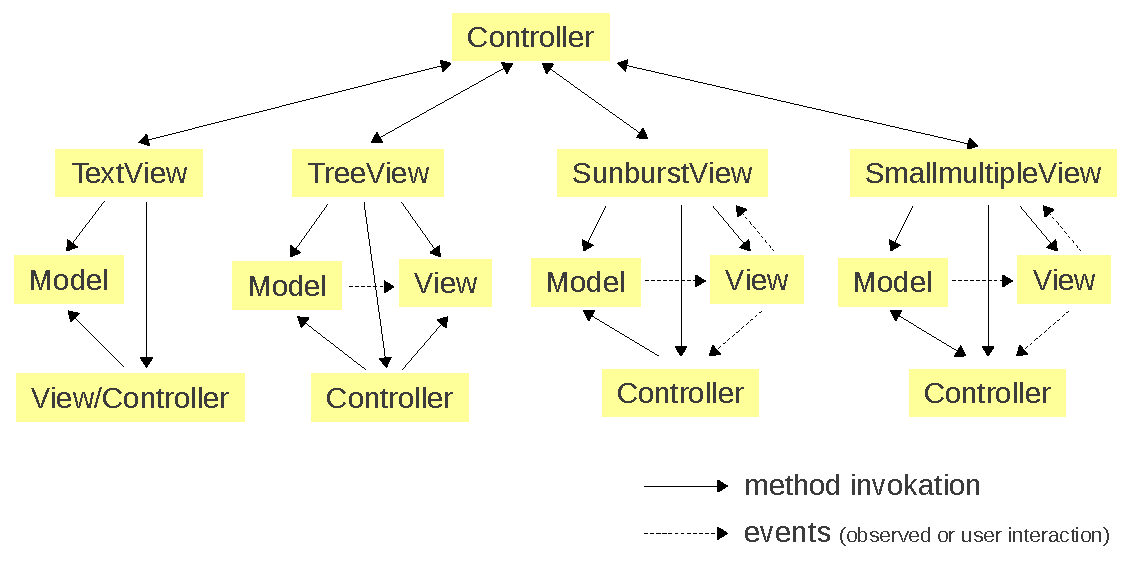
\includegraphics[width=\textwidth]
{figures/mvc}}
\caption{\label{fig:mvc} MVC-paradigm use. The \emph{TextView} and the \emph{TreeView} use standard Swing components. A \texttt{JTree} Swing-component is used implement the tree-model in the \emph{TreeView}. A \texttt{JTreeCellRenderer} implements the view and controller. It is responsible to translate user actions and to render the cells appropriately. The \texttt{JTextEditPane}-Swing component represents both the view and controller in the \emph{TextView} whereas a new \texttt{StAXDiffSerializer} described later on implements the \texttt{XMLEventReader} StAX interface to support a pull based API. It is thus the model which interacts with Treetank through a open database handle.}\end{figure} 

\subsection{Aggregation}\label{subsec::aggregation}
An aggretion of two tree-structures is illustrated in Fig. \ref{fig:aggregation}. The top half depicts the two tree-structures (revision 1 and revision 2) to compare whereas the bottom displays the aggregation or fusion of the trees based on diff-tuples encountered by the internal ID-based diff-algorithm. The two trees are input to the ID-based diff-algorithm which in turn fires diff-Tuples. These tuples form the basis of the agglomerated tree-structure. A straight forward approach which we followed is to store the tuples in a simple List datastructure \footnote{in our case a Map which is used like a List to exchange a Java core collection map implementation with a persistent BerkeleyDB map implementation}. The colors of the nodes in the agglomeration denote if and what change is made. Deletions for instance are marked in red, whereas insertions are colored blue. All update-operations of the ID-based diff-algorithm in Chapter \ref{sec::differences} are supported. Updates are not only supported for leaf nodes, as in the ContrastTreemap approach described in Chapter \ref{sec::relwork} but also for internal nodes. Furthermore the replace-operation as well as moves are supported. Move operations are plotted via curves using hierarchical edge bundles which are drawn on top of the Sunburst layout, whereas an item indicating the position in the old tree-structure (\texttt{DiffType.MOVEDFROM}) and another item denoting the position in the other tree-structure (\texttt{DiffType.MOVEDTO}) is drawn. Items which represent updated nodes include both the value from the first tree and the value from the second tree. Items which constitute replaced nodes include the value from the replaced node as well as the new node. Note that this operation is useful if comparing temporal tree-structures which change over time. The aggregation is automatically achieved through the usage of the ID-based internal diff-algorithm. The model is registered as an observer and the changes are added to a List which is a parameter of a special diff-axis to create the Sunburst Items for the new comparsion layout.

\begin{figure}[tb]
\center{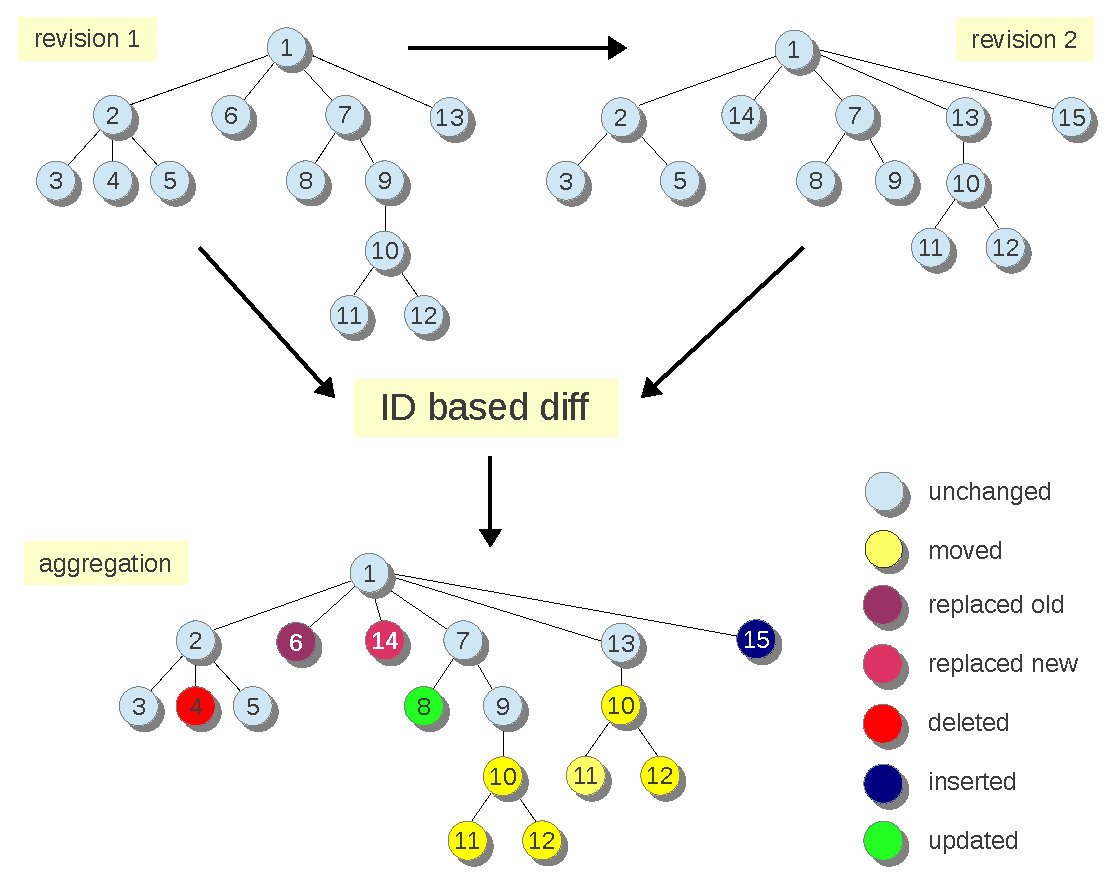
\includegraphics[width=\textwidth]
{figures/aggregation}}
\caption{\label{fig:aggregation} Two tree-structures aggregated. The numbers denote unique node-IDs and refer to Fig. \ref{fig:diff} in Chapter \ref{sec::differences} just like the changes from revision 1 to 2. Both revisions are input to the ID-based diff-algorithm. The output represents diff-tuples including the node-IDs from both nodes which are compared in each step, the type of diff and the depths of both nodes. Storing the observed diff-tuples in an ordered data-structure forms a tree-aggregation.}
\end{figure} 

\subsection{Visualizations}
Visualizations are a major contribution in this thesis. As described in the motivation humans are best in interpreting visual content. Therefore visualizations have been developed which facilitate humans in gaining new insights and quickly detecting differences in tree-structured data. Next, all available views are described in detail. %An XML based serializ   ation view of the tree-structure   %A few of them currently only support the visualization of one revision of the tree-structure. While not being of exceptional value for comparing trees besides viewing two instances of the GUI side by side they will most probably be extended to support

\begin{itemize}
\item
First, a \emph{TreeView} displays nodes in a tree structure just like visual frontends for filesystems as illustrated on the left side in Fig. \ref{fig:treetextview}. Nodes can be expanded to show all child nodes which are inside the current viewport or collapsed to hide children. Therefore a Java-Swing \texttt{JTree} is used which has been extended to mark the subtree of a selected node with a background color. The \texttt{TreeCellRenderer} renders nodes according to their node type and a \texttt{TreeModel} interacts with the storage. Currently the view is not able to incorporate the differences encountered via the diff-algorithm and therefore not further described.

\begin{figure}[tb]
\center{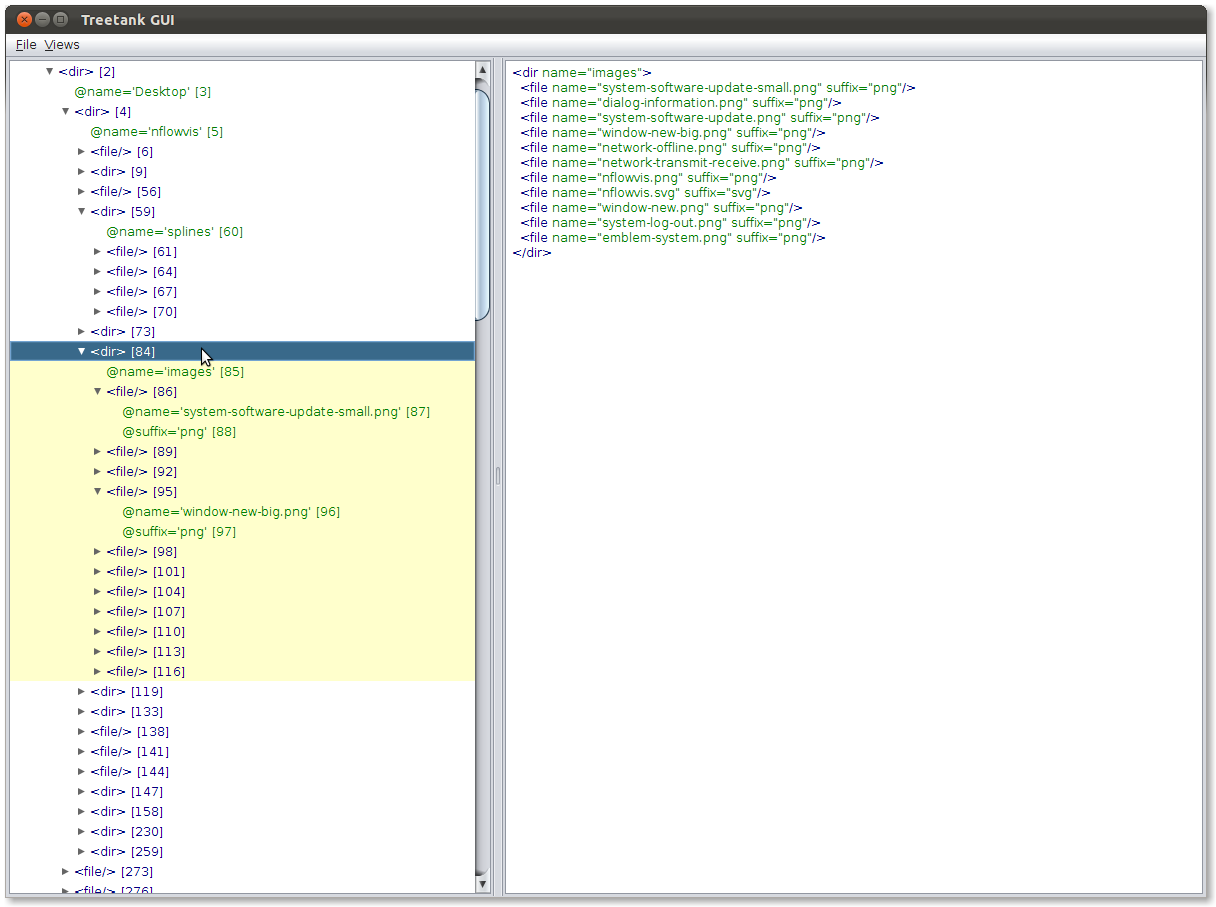
\includegraphics[width=\textwidth]
{figures/treetext}}
\caption{\label{fig:treetextview} TreeView and TextView side-by-side}
\end{figure}

\item
The \emph{TextView} displays serialized XML-documents or fragments and supports syntax highlighting. Moreover it just serializes the part of data which is currently viewable and an additional small overhead of pixels to enable scrolling. Other data is serialized and appended to the text pane once a user scrolls down. A new \emph{StAX}-parser implementation provides a pull-based API to support this "append-on-scroll" behaviour. It provides two features. Since it is pull based the application (the GUI) can determine when and how much data is parsed. Furthermore it provides the parsed node kinds which are used to support syntax highlighting. Simply using a \texttt{DescendantAxis} from Treetank which traverses the nodes in preorder would not be sufficient, end-tags have to be emitted as well. Therefore it is much easier to develop a reusable \texttt{StAX}-implementation. Nontheless the \texttt{DescendantAxis} is used internally as part of the implementation to traverse the tree in preorder. The algorithm which implements a StAX-Parser for Treetank is outlined in appendix \ref{Algorithm}. To adhere to the specifications of the methods which must be implemented and to keep the iterator-methods idempotent might have been the biggest challenge. In addition to generate events for end-tags the StAX-parser supports a \texttt{peek()}-method.

Figure \ref{fig:treetextview} displays the \emph{TreeView} and the \emph{TextView} side by side. Note that the two views are kept in synchronization.

In order to support an analyst with the task of analysing differences in tree-structured the view supports another mode which incorporates the aggregation of the two tree-structures to compare described in section \ref{subsec::aggregation}. Based on this aggregation another StAX-Parser called \emph{StAXDiffSerializer} has been developed which receives a \texttt{DiffAxis} to iterate over \texttt{SunburstItems} created for the \emph{SunburstView} which is described next. We support a preorder-traversal of the items to derive the stored diff-types as well as the depths in the items without the distortion of a semantic view for the \emph{SunburstView} described later on in this chapter. The depth of the current item and the depth of the next item using a \emph{peek()} method on the \texttt{DiffAxis} are used to determine if an end-tag must be emitted. Another check involves empty-Elements whereas an \texttt{EndElement} must be emitted immediately following the \texttt{StartElement} in the case of the next call to \texttt{nextEvent()}. In this case the parent node-IDs must match. Furthermore the depths are used in subsequent calls to \emph{nextEvent()} to determine how many closing tags must be emitted. In case of \texttt{ElementNode} updates we immediately emit the new updated element and push the old element on an end-tag stack. In a subsequent call to \texttt{nextEvent()} the old value in case of a \texttt{TextNode} or the old element in case of an \texttt{ElementNode} are emitted. Changed nodes are highlighted with a background color which denotes the kind of change. The \texttt{TextView} itself must not change the indentation for the old value/old element if an UPDATE has been detected. Only the first emitted value (the new value) must change the indentation. 

A legend which describes the color $\leftrightarrow$ change mapping is currently only available from within the \emph{SunburstView} which is described next. However this is only an implementation detail and a help-dialog can be added easily. Exemplary a side-by-side view with the \emph{SunburstView} is depicted in Fig. \ref{fig:sunbursttextview} whereas the first inserted subtree is also visible in the \emph{TextView} area. Note that while the SunburstView provides a great overview about the whole tree-structure and subtrees, the \emph{TextView} provides a better detailed view on selected parts of the whole tree-structure. Other deficiencies meantioned in the introduction regarding the boundary of nodes and XML-specific details do not apply as we compare the tree-structure, instead of a character based comparsion, with the ID-based diff-algorithm in the first place. Besides the lack of an appropriate overview, which is one of the advantages of the \emph{SunburstView}, the \emph{TextView} is an ideal partner to the \emph{SunburstView} as the XML text-serialization is better readable than radial Sunburst labels and readers might be more familiar with pure XML.

Note that the diff-algorithm is only ever called once for every visible view (besides a smallmultiple variant which represents changes among several tree-structures or revisions in Treetank), whereas a simple iterator on the created \emph{SunburstItem}s is broadcasted to all other views which are currently visible to support the iteration over the agglomerated tree-structure.

\begin{figure}[tb]
\center{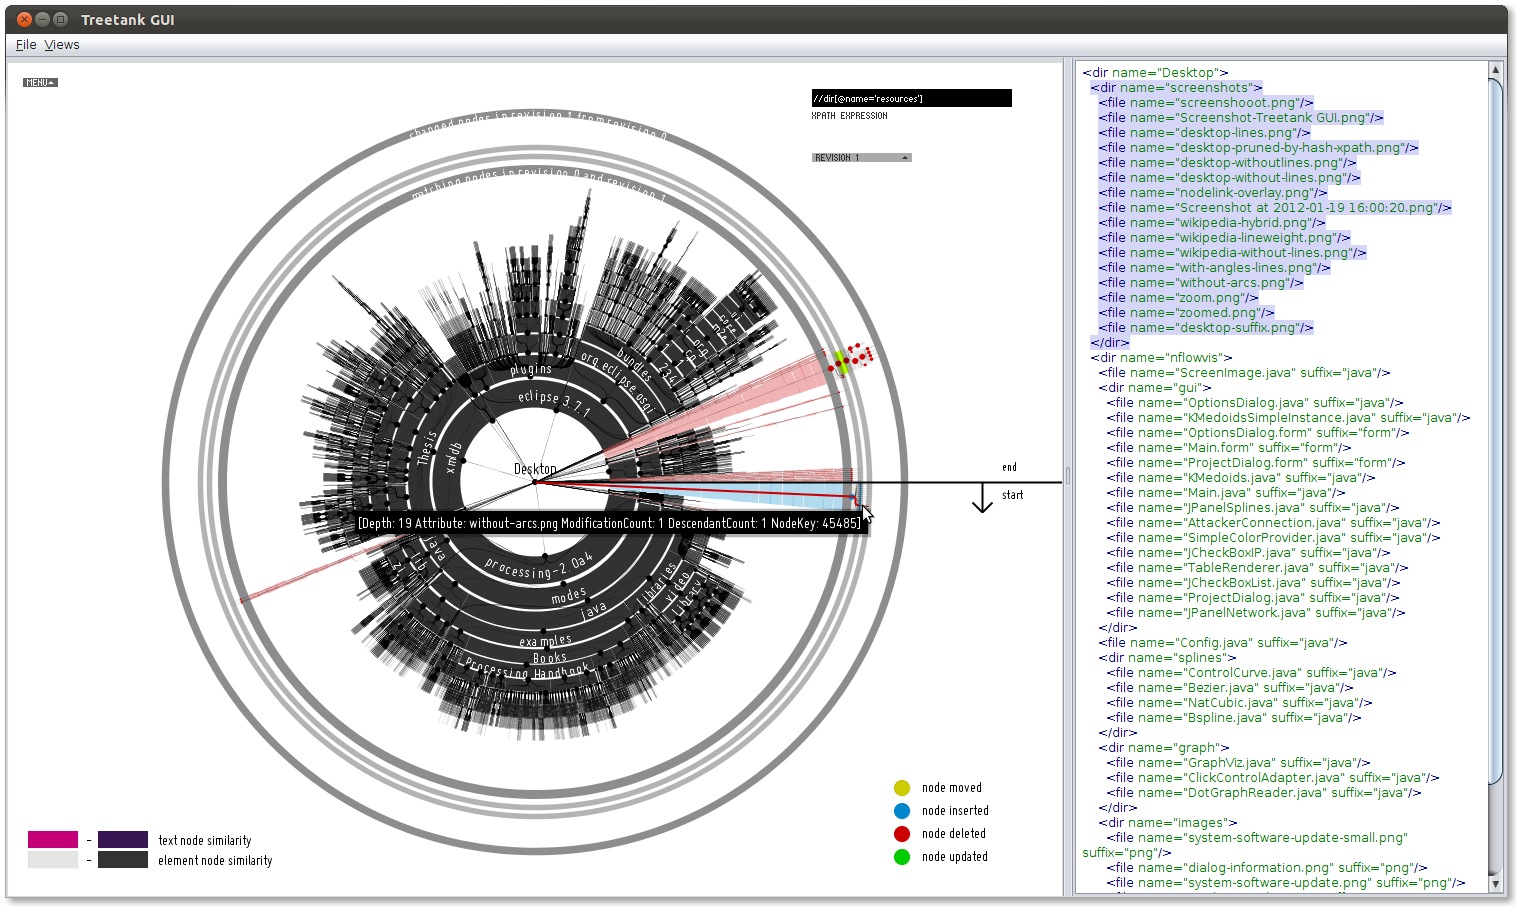
\includegraphics[width=\textwidth]
{figures/sunbursttextview-overview}}
\caption{\label{fig:sunbursttextview} SunburstView and TextView side-by-side}
\end{figure}

\item
The \emph{SunburstView} displays the tree structure in a radial arrangement. It is a space filling approach which tries to maximize available screen space for the hierarichical visualization. Furthermore it is adjacency based drawing child nodes next to their parent node. In contrast Treemaps enclose child-nodes within parent nodes. Thus a Treemap utilizes available screen space to the full extend as the root node uses all available space recursively embedding descendants as rectangles. In the Sunburst method unlike in Treemaps the corners are left empty due to the radial representation. While this alone on first glance might be a great drawback in addition to circular segments which are more difficult to read regarding size and the labels, the layout is stable even with a lot of changes and the hierarchical structure is much better readable. The Spiral Treemap layout which has been described in chapter \ref{sec::relwork} is relatively stable but it is still very difficult to track changes which might be scattered through a 45° degree change in direction as well as the complicacy to follow nested rectangles which are arranged in spirals compared to the simplicity of a Sunburst layout.

The root node of a tree-structure is plotted in the middle of the screen depicted as a circle. Child-nodes of the root node are plotted in circular segments next to their parent. In our case the radius depends on the depth and shrinks for an increasing depth such that the full circular area between two levels does not change. Otherwise items toward the edged will occupy more space. However this behaviour can be changed which is of importance to visualize changes which will be visualized along the edge (section \ref{subsec::comparison}). The extend of an item in the Sunburst layout which depicts one node depends on an attribute of the node whereas a relative measure in regard to the other children is used.  

The \texttt{SunburstView} is displayed in Fig. \ref{fig:sunburstview}.

\begin{figure}[tb]
\center{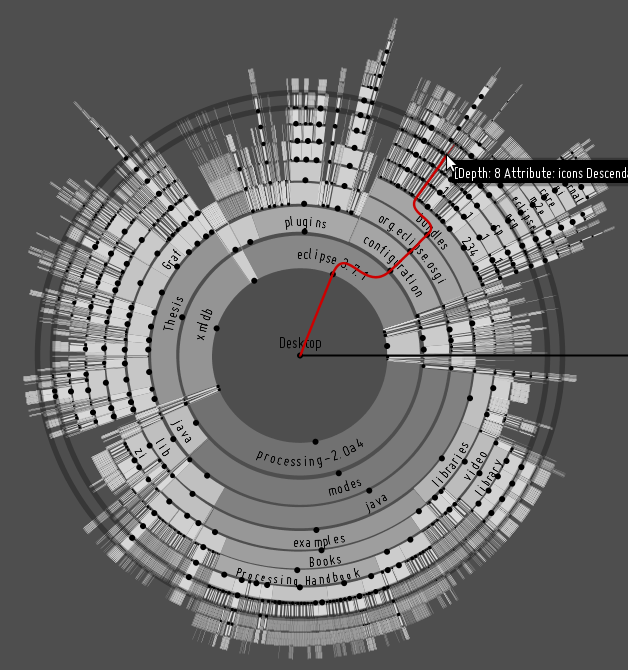
\includegraphics[width=\textwidth - 5em]
{figures/sunburstview-cut}}
\caption{\label{fig:sunburstview} SunburstView}
\end{figure}

The number of descendants of a node plus one is mapped onto the extend of each segment such that nodes having more descendants have a greater arc and therefore get more space. The formular is straight forward:

\begin{equation}
ext = \left\{ \begin{array}{cl}
2 \cdot \pi & \textrm{if }node\ is\ root\ node\\
parExt \cdot descs / (parDescs - 1) & \textrm{otherwise}\end{array}\right.
\end{equation}

Note that recently we have added the number of descendants of each structural node in Treetank itself to maximally speed up the creation of the visualization. Before, while creating the items we issued a preorder traversal on each node in parallel using the Java \texttt{ExecutorService} and a \texttt{BlockingQueue} which is also used in the comparsion view described later.

%\begin{equation}
%currExt = parExt * descCount / parDescCount
%\end{equation}

The color of each segment in case of internal nodes (element nodes) is mapped to the number of descendants of a node plus one as well. Having that said in future versions it will be possible to map another custom attribute available through a drop-down menu to the color. If such an attribute is not available for every node a default value can be assumed. Leaf nodes which are \texttt{text-nodes} are colored according to their text-length.

A node-link diagram is drawn on top of the \emph{SunburstView} to further emphasize the hierarchical structure. Dots representing the node in addition to the SunburstItem-segments are depicted in the middle of the segment whereas either bezier curves or straight lines denote a child/parent-relationship between the nodes.

In order to support large tree-structures the generated Sunburst-segments are drawn into an offscreen buffer, whereas the actual items are only used to implement a mouseover effect and to enable XPath-queries and highlighting of result-nodes.

\subsubsection{Interaction}
The view is highly customizable. Through checkboxes the dots/circles and/or the arcs can be hidden as well as the radius of the arcs can be adjusted through sliders. Moreover the size of the dots can be managed through a slider, whereas the connections between child/parent-nodes in the node-link overlay either can be disabled or a range denoting the line/curve thickness is adaptable. By default links at a higher level are drawn in thicker depending on the range. Furthermore color values for thecan be changed for the arcs , the background color, which also automatically adjusts legend text-colors to white if the background-color is very dark. On top of that it's possible to adjust the values such that either the whole node-link diagram or the \emph{SunburstView} disappears. Some adjustments are depicted in Fig. \ref{fig:sunburst-adjusted-scale}.

\begin{figure}[tb]
\center{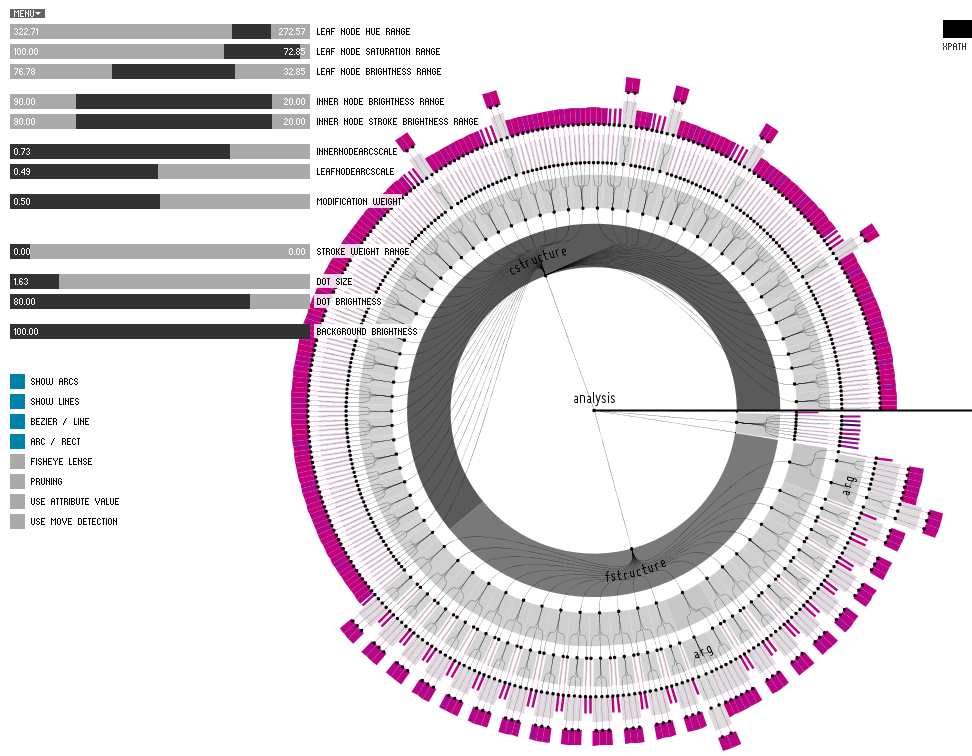
\includegraphics[width=\textwidth]
{figures/sunburst-adjusted-scale-cut}}
\caption{\label{fig:sunburst-adjusted-scale} SunburstView - adjusted arcs/dotsize parameters}
\end{figure}

Figure \ref{fig:nodelink} illustrates the node-link overlay without coloring the arcs. The red curve marks a path up to the root-node through all ancestor-nodes for the current node which is highlighted by moving the mouse over the item.

Besides, mapped values to the color of Sunburst-segments or items, a term which is used interchangeably in the following sections, can be normalized according to a linear, squareroot or logarithmic scale.

\begin{figure}[tb]
\center{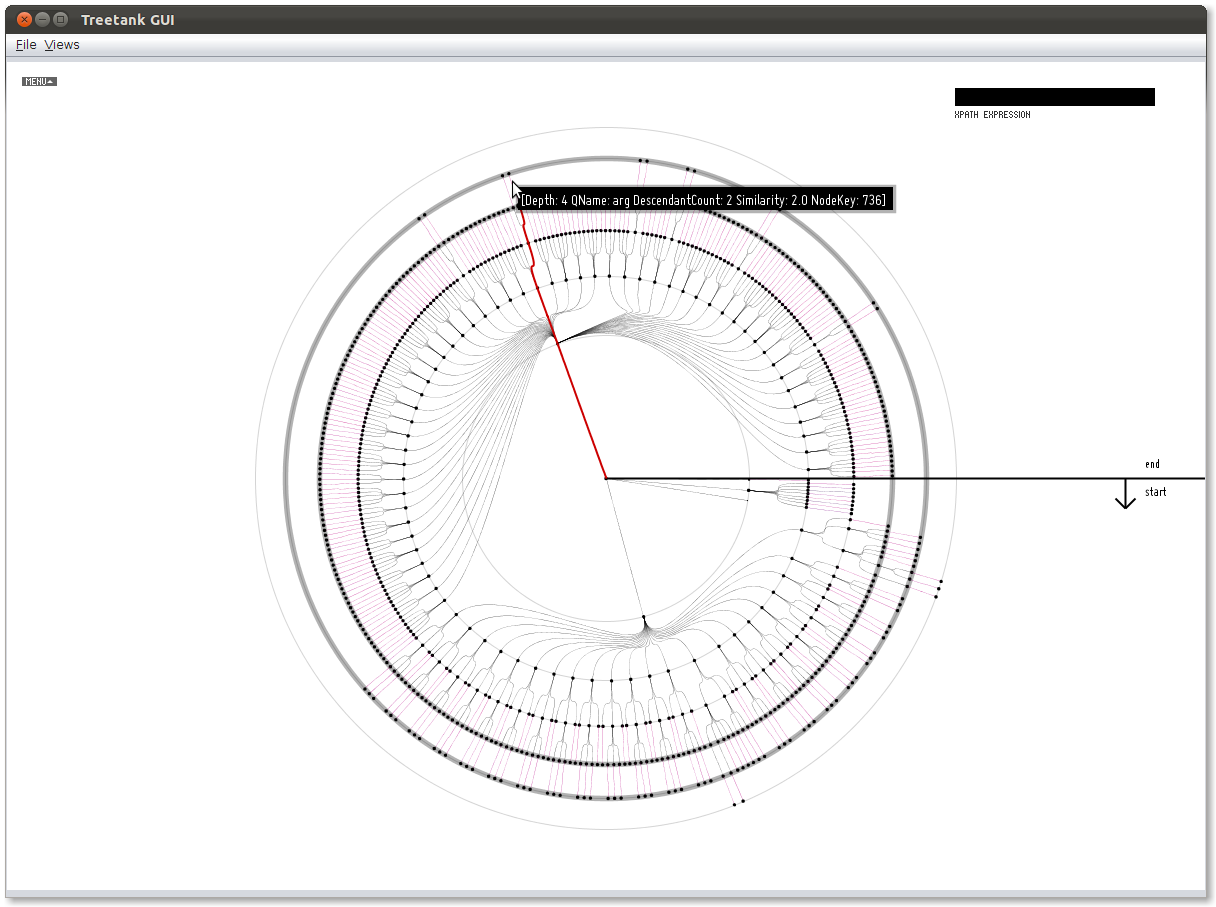
\includegraphics[width=\textwidth]
{figures/nodelink}}
\caption{\label{fig:nodelink} node-link diagram}
\end{figure}

Crucial to the interaction and the value of the visualization itself is the possibility to drill down into the tree. Clicking an item results in drawing the selected node with its subtree in a new Sunburst-diagram whereas the selected node is simply used as the new root-node. Stacks are used to implement a simple undo-operation which is very fast as we store the Sunburst-items as well as the background buffer-image. 

A well known technique to enlarge small regions is to use transformations of the screen-space, as for instance a fisheye lense. The enlargement of small items via a fisheye lense is depicted in Fig. \ref{fig:fisheye}. Zooming and panning is also incorporated allowing affine transformations of the screen (Fig. \ref{fig:zoom}) to analyse important regions. Note that the mouseover-effect displaying additional information about the node itself as well as the legends are not affected by the transformation. As the background-buffer cannot be used in this case zooming is restricted to smaller trees with an upper bound of about 10\_000 to 15\_000 nodes.

\begin{figure}[tb]
\center{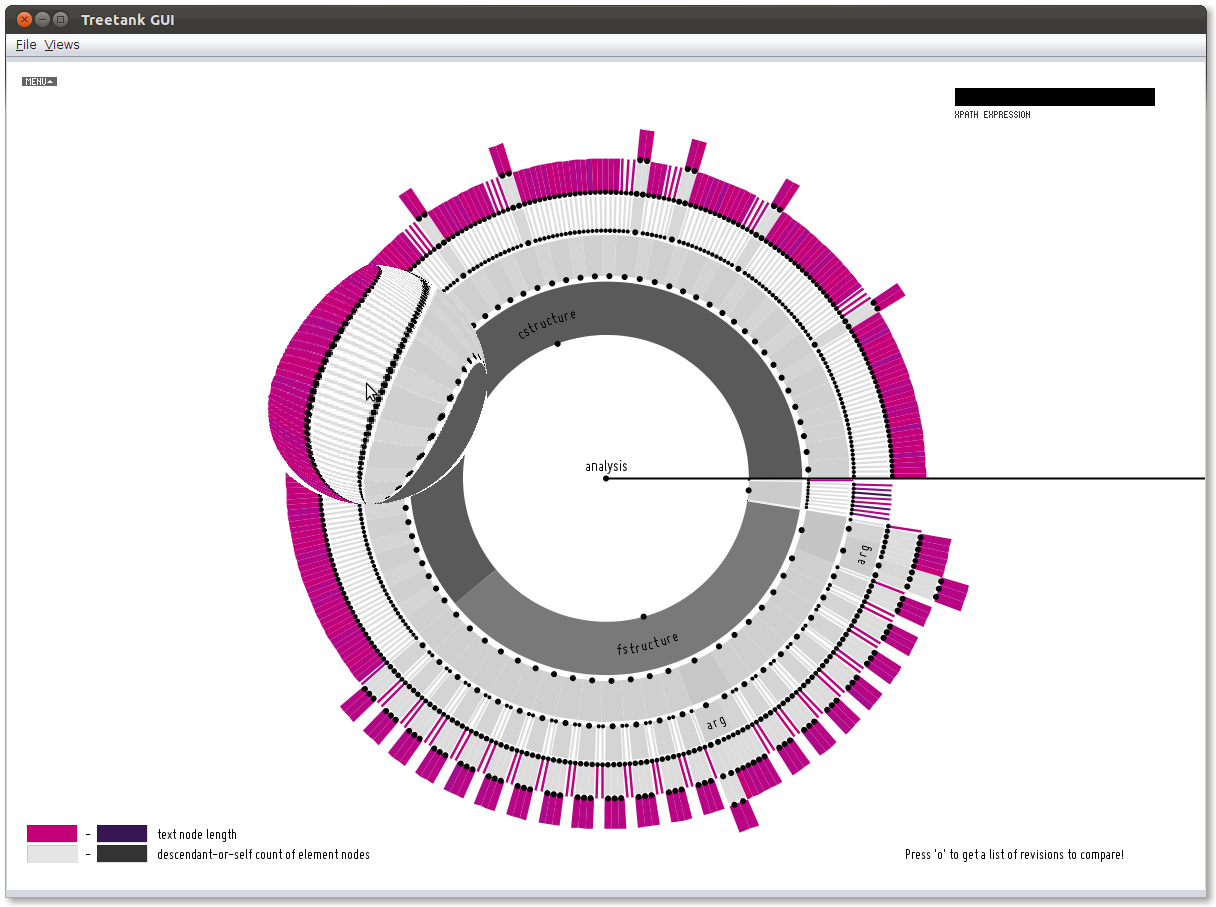
\includegraphics[width=\textwidth]
{figures/fisheye}}
\caption{\label{fig:fisheye} Fisheye transformation}
\end{figure}

\begin{figure}[tb]
\center{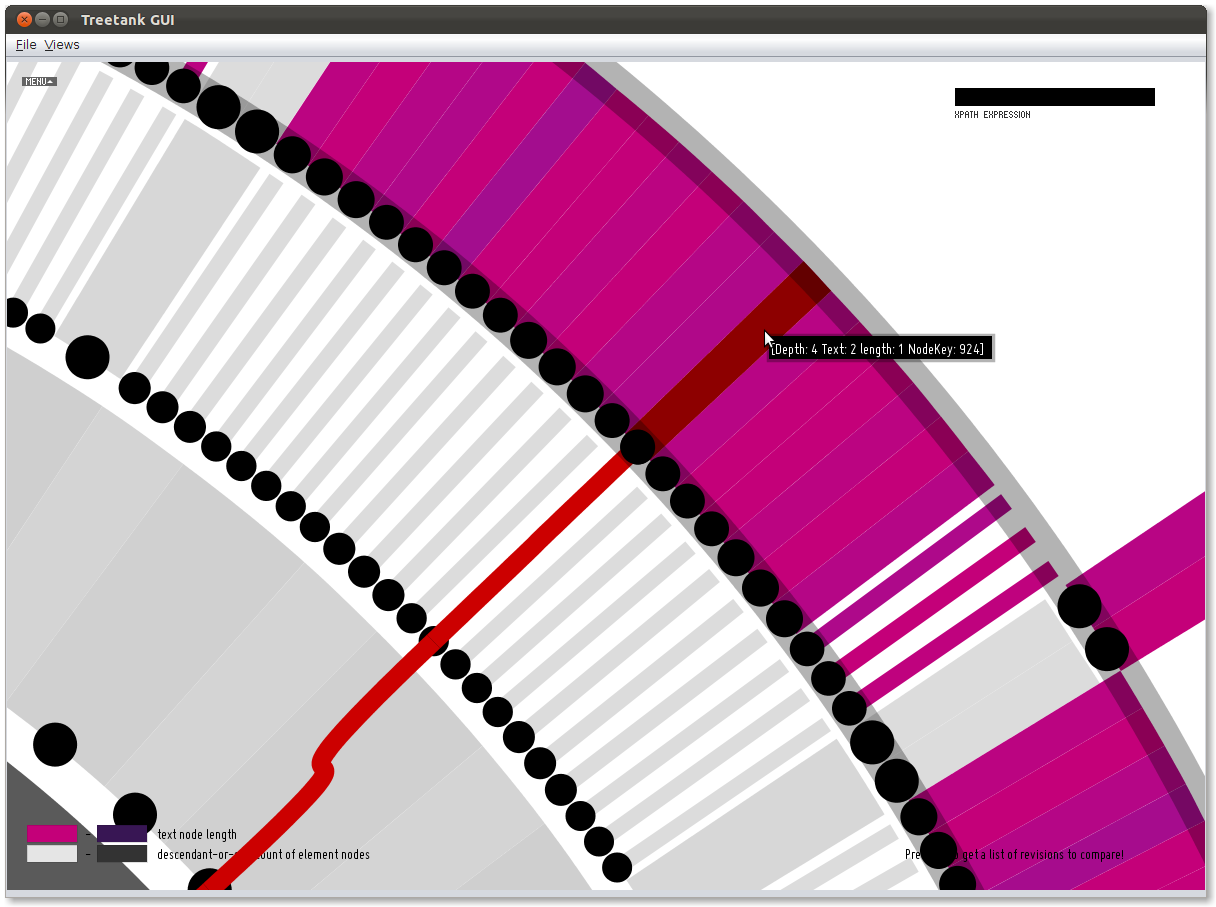
\includegraphics[width=\textwidth]
{figures/zooming}}
\caption{\label{fig:zoom} Zooming into the visualization}
\end{figure}

In order to manipulate Treetank resources it is even possible to insert XML fragments as right-siblings or first-childs as well as to delete nodes.

\subsubsection{Querying}
XPath can be used to query the tree-structure for specific nodes. Result sequences are highlighted in a light green. Figure \ref{fig:sunburstxpath} displays the result of a simple \texttt{//*[text()='var:0']} query to highlight all nodes which have a text-node child with the value "var:0".

\begin{figure}[tb]
\center{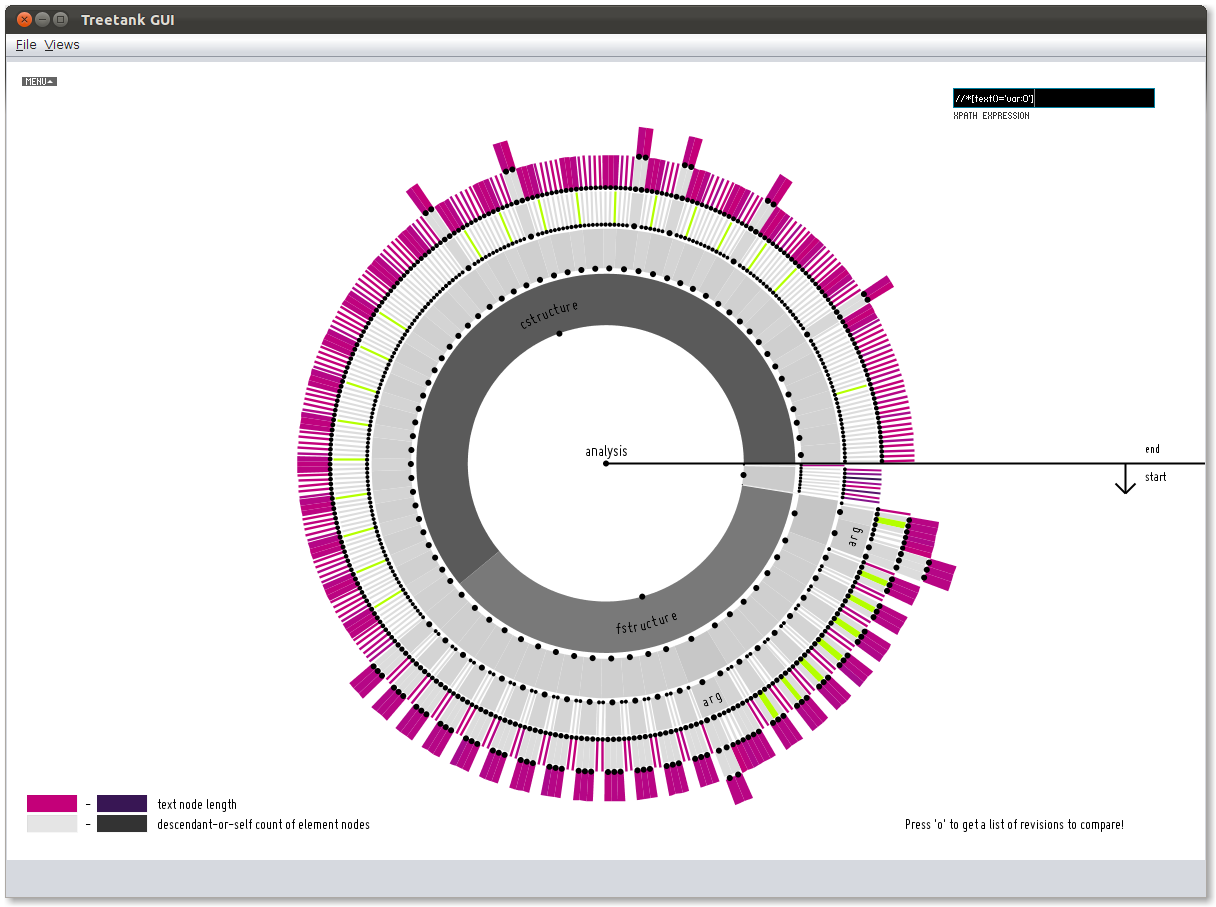
\includegraphics[width=\textwidth]
{figures/sunburstxpathquery}}
\caption{\label{fig:sunburstxpath} XPath query results displayed in light green}
\end{figure}

\subsubsection{Labels}
If the Sunburst items are huge enough and the scale to draw the arcs for each depth is greater than a predefined value (currently 0.7, whereas the scale ranges from 0 to 1) labels are drawn. Labels in the top half of the visualization, that is if the center of the item is greater than $\pi$, are drawn beginning at the startAngle in clockwise direction, otherwise they are drawn starting from the endAngle in counter clockwise direction. Furthermore the font-size ranges between two values, whereas the size is decreased with an increasing level. 

\subsubsection{Filtering/Pruning}
The standard \emph{SunburstView} incorporates a method to filter the tree by level. While this filtering is not perfect in circumstances where the fanout is very large, it turned out to work very well to keep the number of generated Sunburst items small. Furthermore the view currently is used as an entry point to the comparsion view which is also based on the Sunburst-layout whereas it is planned to backport the filtering by itemsize. In the following we use the terms \emph{filtering} and \emph{pruning} interchangeably.

Whereas it will be sufficient to use an XPath-query as for instance \\
\texttt{//*[count(ancestor::*)<3]} to get a sequence including all nodes between level 0 and 3 we opted for a tree-traversal implementation, as the XPath query has to touch all ancestor nodes in the current Treetank implementation which doesn't incorporate hierarchical node-IDs as for instance the ORDPATH/Dewey-IDs where it's usually trivial to compute such queries on the ID itself in an in-memory B*-tree or something alike. To support such queries efficiently it is scheduled to include the depth for each inserted node, which usually doesn't have to be adjusted in case of all operations but the movement of nodes/subtrees. In that case all moved nodes have to be adjusted instead of just the root node and it's former siblings/parent and the new siblings/parent. Furthermore the \texttt{DescendantAxis} and/or \texttt{VisitorDescendantAxis} can be adjusted to optionally use a maximum depth for the traversal.
\end{itemize}

\subsection{Comparsion using a new Sunburst-layout algorithm}\label{subsec::comparison}
The standard \emph{SunburstView} includes a comparison-mode. Once a base revision is opened and the \emph{SunburtView} is enabled an analyst is able to choose another revision from a dropdown menu for comparison. Note that all interaction capabilities described earlier are also available in the comparison mode. Differences and additional capabilities are described in the following sections. In order to compare tree-structures in a radial arrangement similar to the described "usual" SunburstView to explore a single revision a new layout-algorithm has been developed. Next, we first describe the new layout.

\subsubsection{Sunburst Comparsion-Layout}
The Sunburst comparison layout is illustrated in Fig. \ref{fig:sunburst}. Nodes are colored as depicted in the color legend in the bottom right corner. All nodes which have not changed as part of comparing the base revision to another revision\footnote{in this case revision 1} are plotted inside the inner circle which is labeled "matching nodes in revision 0 and revision 1". The circle itself is drawn between the maximum level of the unchanged nodes plus one and maxLevel plus two. Changed nodes are zoomed out from their original place and drawn between the two dark circles labeled "changed nodes in revision 0 and revision 1" and "matching nodes between revision 0 and 1". To demonstrate the area denoting the changes it is hatched in Fig. \ref{fig:sunburst}. Similarly the arrows emphasize the direction in which changed subtrees are zoomed/dislocated. This semantic zoom serves a double purpose. First, the visualization adheres to a Tree-Ring metapher depicting the evolution of a tree. Like the age of a tree in the nature is deducable by analysing rings in a cross-cut of the stem whereas the rings denote the age and each ring represents one year starting from the very middle to the outside, our representation aims at representing the changes between two rings. In our representation the unchanged nodes form the middle of the \emph{SunburstView} whereby changed nodes are zoomed to the border between the outer and inner ring which is representing the growth of a tree in case of analysing temporal tree-structures. Additionally this transformation of changed subtrees displaces these subtrees to a prominent place. Small changed subtrees are thus much better noticeable as they are not surrounded by unchanged subtrees which might even be deeper. To depict changes between multiple trees first considerations involved the addition of changes from a sequence of sorted revisions in further circles around the one denoting the changed nodes. That is, the inner circle represents unchanged nodes between \emph{all} compared revisions whereas changes between selected or consecutive revisions are drawn between new outer rings which are appended. According to the Tree-Ring metapher each comparison between a pair of trees would append a new rings for their changes. However this would affect the whole layout each time. The idea proved to be not viable because of the complexity this involves. To name a few

\begin{itemize}
\item The inner ring must keep space between unchanged nodes/subtrees for all changed subtrees in the outer rings.
\item Consecutive calling the diff-algorithm and merging diffs into a diff-list with diff-tuples which has already been created.
\item Keeping track of all opened transactions and resetting the transaction appropriately depending on the revision in which a change has occured.
\item Similarly the depth for items in the tree will change very often which involves further state and it is almost not possible to denote the current depth.
\item The \texttt{descendant-or-self}- and \texttt{modification}-count of each nodes' subtree will be cumbersome to calculate.
\end{itemize}

\begin{figure}[tb]
\center{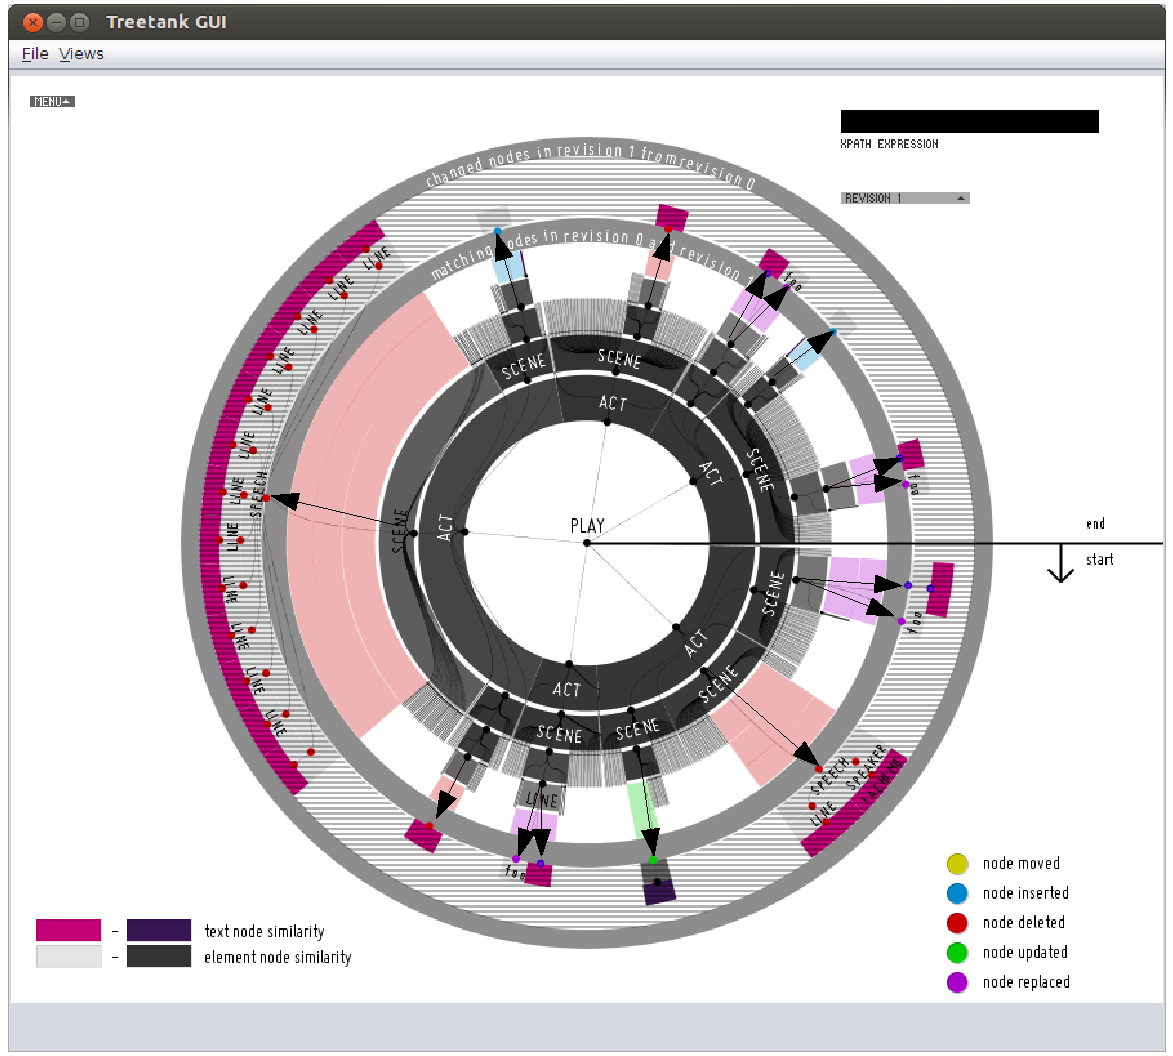
\includegraphics[width=\textwidth]
{figures/sunburst.pdf}}
\caption{\label{fig:sunburst} SunburstView - comparison mode.}
\end{figure}

These and similar complexity considerations formed the idea of introducing Small multiple visualizations of the current view which are described in section \ref{subsec::smallmultiple}.
Adhering to the Tree-Ring metapher, the semantic zoom surves the purpose that all changed nodes are visible on first glance. Otherwise it would be hard to track small changes. 

\subsubsection{Short animation}
In order to clearly demonstrate the semantic zoom a short animation has been implemented as test persons usually did not grasp the meaning without further explanation. Thus the transformation of changed subtrees is shown which dislocates the items to their dedicated positions along the arrows in Fig. \ref{fig:sunburst} \footnote{remember, the arrows are not drawn in the visualization, they have been added to the screenshot to emphasize the transformation}. However the animation is only drawn if the framerate will not drop due to too many items. Thus when a certain amount of items has been created the animation will be skipped.

\subsubsection{Layout algorithm}
After invoking the ID-based diff-algorithm depending on the chosen filtering-method (described in the next section) the new Sunburst-layout has to be drawn. First of all, based on the generated aggregation of the trees, Sunburst items which denote the nodes in the aggregated tree have to be computed. The diff-tuple encountered through observing changes computed by the ID-based diff-algorithm is of the following form: key in first revision / key in second revision / depth in first revision / depth in second revision / kind of diff. The Sunburst items are created based on a special axis which implements the Iterator/Iterable interfaces from Java to traverse the diff-tuples. That is the following two methods are available: \texttt{hasNext()} and \texttt{next()}. Initially we developed an axis based on the idea of traversing the tree-structure just like in the \texttt{SunburstDescendantAxis} and to adjust a simple index-variable pointing to the next diff-tuple. The key idea is to traverse the tree-structure based on the transaction opened on the newer revision whereas usually the pointers of the nodes are used as a guidance to traverse the aggregated tree-structure in document-order. The transaction will be changed to the old revision whenever a diff of type \texttt{DiffType.MOVEDFROM}, \texttt{DiffType.DELETED} or \texttt{DiffType.REPLACEDOLD} is encountered. However the preorder-traversal using a pointer-based approach similar to the algorithms in the \texttt{SunburstDescendantAxis} or the \texttt{DescendantAxis} itself bares a lot of complexity as the node key of the next node to traverse has to be set in advance and the movement of the transaction in a lot of cases cannot be immediately reflected by adjusting certain stacks which are required to determine the start-Angle, extend, descendantCount, modificationCount and the parent index. In fact in some cases the adjustments can not be done until the next call to \texttt{hasNext()}. Figure \ref{fig:tree-axis} demonstrates a lot of this complexity on a simple tree-aggregation. Note that the terms "aggregation" and "agglomeration" are used exchangeable in this thesis. 

\begin{figure}[tb]
\center{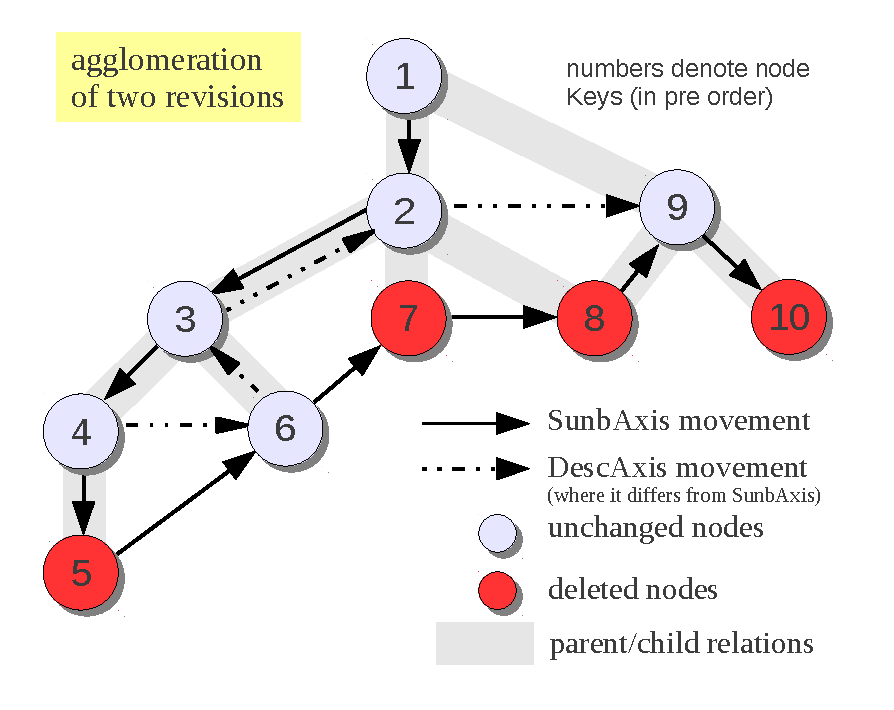
\includegraphics[width=\textwidth - 12.5em]
{figures/tree-axis}}
\caption{\label{fig:tree-axis} SunburstCompare-Axis based on the Sunburst-Axis}
\end{figure}

If the transaction-cursor is located at the node with the nodeKey 4 in the new revision the next nodeKey will be the node denoted by nodeKey 6 in the \texttt{Descendant}- and the \texttt{Sunburst}-axis as node 5 is deleted. As such the simple expression $rtx.getStructuralNode().hasFirstChild()$ to test for a child node must be extended to keep track of these issues, for instance by receiving the next element in the diff-list and compare the diff to the type \texttt{DELETED} and \texttt{MOVEDFROM} whereby the depth must be greater than the current depth. Furthermore the kind of movement must be tracked just like in the \texttt{SunburstDescendantAxis} to adjust the stacks with the start-angle, extension, depths and descendant- as well as modification-number accordingly. Everytime before a new SunburstItem is added to a list which contains all resulting items in the end, the values as for instance the descendant-or-self number and the modification-number as well as the startAngle/extension must adapted based on the stacks which have to be adjusted themselfes depending on the transaction movement. 

Another example of the complexity is the movement from node 6 to node 9 in the normal \texttt{DescendantAxis} whereas in our case the next node is the deleted node 7. Thus the \texttt{pop()}-method on the stacks must be called once instead of two times. Each time a \texttt{DELETED} or \texttt{MOVEDFROM} diff kind is encountered the transaction is temporarily changed along with the nextNodeKey which denotes the key the $hasNext()$-method must move to the next time called and a right-sibling node stack which is used in cases where the node has no first child and no right sibling. In this case the next nodeKey is popped from the right-sibling stack (a nodeKey is pushed on the stack for each child-movement whenever the node before the move to the first child has a right sibling) and as in the algorithm \ref{algo:popStacks} the depth must be considered too, that is like in the example scenario described before such that the pop()-method is called the right number of times. This method is invoked for the first \texttt{DELETED} or \texttt{MOVEDFROM} after another diff-kind has been encountered. If the movement of the transaction before calling this method was of kind \texttt{EMoved.ANCHESTSIBL}, that is the transaction will be moved to the right sibling of the first ancestor which has one. This cannot be done until the next call to $hasNext()$ as otherwise the stacks will not be adapted appropriately. Note that the first while-iteration doesn't call pop() as no values have been pushed on the stacks for leaf-nodes. Another remark concerns the else-branch which is executed if the depth of the current node in the list is equal or even greater than the last depth.

Similarly if the movement-type was to a right sibling of the first anchestor-node which has one and the next node will not be of the kind \texttt{DELETED} and \texttt{MOVEDFROM}, the actual movement cannot be done before the next call to $hasNext()$ and the method is very similar to algorithm \ref{algo:popStacks}.

\begin{algorithm}[Hhtbp]
%\SetAlgoLined
\SetKwInOut{Input}{input}\SetKwInOut{Output}{output}
\Input{instance variabled denoted by a trailing m, int initDepth, Diff lastDiffCont, EMoved moved}
\Output{nothing, the instance variables are directly modified (method/algorithm has side effects)}
\BlankLine
int tmpDepth = 0\;
\If{mDepth == 0}{
  tmpDepth $\leftarrow$ initDepth\;
}\Else{
  tmpDepth $\leftarrow$ lastDiffCont.getDepth().getNewDepth()\;
}
\If{mMoved == EMoved.ANCHESTSIBL}{
  \If{tmpDepth - mInitDepth $>$ diffCont.getDepth().getOldDepth() - initDepth} {
    \tcp{Must be done on the transaction which is bound to the new revision.}
    boolean first $\leftarrow$ true\;
    \While{tmpDepth - initDepth $>$ diffCont.getDepth().getOldDepth() - initDepth} {
      \If{first == true}{
        \tcp{Do not pop from stack if it's a leaf node.}
        first $\leftarrow$ false\;
      }\Else{
        mDiffStack.pop()\;
        mAngleStack.pop()\;
        mExtensionStack.pop()\;
        mParentStack.pop()\;
        mDescendantsStack.pop()\;
      }

      tmpDepth--\;
      mDepth--\;
    }
  }\Else{
    moved $\leftarrow$ EMoved.STARTRIGHTSIBL\;
    mAngle += mExtension;
  }
}
\caption{adjusting stacks and depths for movement to next following node for the first DELETED or MOVEDFROM node after another type has been encountered}\label{algo:popStacks}
\end{algorithm}

The last pitfall in Fig. \ref{fig:tree-axis} is after traversing the node denoted by nodeKey 9. Usually $hasNext()$ will return false but in this case it must return true, as the deleted node "10" follows.

We observed that the overall algorithm is very complex in terms of a lot of special cases as described in the last paragraphs have to be considered which directly results in many comparsions and instructions and therefore might be a performance issue as well.

The complete algorithm therefore is not described as recently a new, in comparsion, lightweight algorithm has been developed. Instead of using a pointer based traversal it became apparent that it is easier to directly use the diff-tuple and move either the transaction on the old revision or the transaction on the new revision depending on the diff-kind. In case of a \texttt{DELETED} or \texttt{MOVEDFROM} the working transaction is based on the transaction opened on the old revision, otherwise the transaction opened on the new revision is used.

The algorithm skeleton for $hasNext()$ is described in \ref{algo:skeleton}.
\begin{algorithm}[Hhtbp]
%\SetAlgoLined
\SetKwInOut{Input}{input}\SetKwInOut{Output}{output}
\Input{instance variabled (denoted by a trailing m)}
\Output{true, if more diffs are in the diff list, false if index == size}
\BlankLine
\tcp{Fail if there is no node anymore.}
\If{!mHasNext}{
  return false\;
}

\tcp{Setup everything.}
setupDiffs()\;

\If{mIsOldTransaction == true}{
  setTransaction(mOldRtx)\;
}\Else{
  setTransaction(mNewRtx)\;
}

\tcp{Move to next key.}
getTransaction().moveTo(mNodeKey)\;

\If{mHasMorDiffKinds == true}{
  \If{mDiff == DiffKind.UPDATED OR mDiff == DiffKind.REPLACEDOLD}{
    \tcp{For DiffKind.UPDATE or DiffKind.REPLACED the transaction needs to be on the right node.}
    mOldRtx.moveTo(mDiffCont.getOldNodeKey())\;
  }

  \tcp{Always follow first child if there is one.}
  \If{mNextDepth $>$ mDepth}{
    return processFirstChild()\;
  }

  \tcp{Then follow right sibling if there is one.}
  \If{mDepth == mNextDepth}{
    return processRightSibling()\;
  }

  \tcp{Then follow next following node.}
  \If{mNextDepth $<$ mDepth}{
    return processNextFollowing()\;
  }
}
\tcp{Then end.}
processLastItem()\;
mHasNext $\leftarrow$ false\;
return true\;
\caption{Diff-Axis hasNext()-skeleton}\label{algo:skeleton}
\end{algorithm}

The method \texttt{setupDiffs} takes care of setting the current depth which depends on the diff-kind/type, the upcoming next depth, if the list has more diff-elements as well as setting the boolean instance variable \texttt{mIsOldTransaction} which is \texttt{true} if the diff-kind is of type \texttt{DELETED}, \texttt{MOVEDFROM} or \texttt{REPLACEDOLD} and \texttt{false} otherwise. After determining which transaction must be used based on \texttt{mIsOldTransaction} if more elements are in the diff-list the transaction is moved to the next key determined by the diff-kind and obtained from the diff-element, the tuple described earlier which incorporates the nodeKey of both nodes which have been compared in the diff-algorithm as well as the depths of both nodes. In order to provide both the old value and new value\footnote{in case of a \texttt{TextNode}} or QName\footnote{in case of an \texttt{ElementNode}} in the case of updates and similarly in case of replaces for the next SunburstItem, the transaction opened on the base revision which is always the older revision is moved to the node key of the node in the old revision. Note that this information is available from the diff-tuple. Thus both transactions are located at the right nodes. The following three \texttt{if}-clauses ensure the preorder traversal of the axis. If the next depth is greater than the current depth the next node is a child node in the agglomerated tree, thus the variables of the last created Sunburst item which depend on the stacks must be pushed on top of these. As in all cases the variable which denotes the movement must be adapted. Otherwise if the next depth is equal to the current depth the next node is a right sibling. In this case the extension of the last emitted Sunburst item has to be added to the startAngle and the movement variable must be adjusted accordingly. Likewise if the next depth is lower than the current depth the next node is a right sibling of the first ancestor which has an appropriate pointer (!= $NULL\_NODE\_KEY$ which denotes that no right sibling is available). Thus the stacks must be adapted similar to algorithm \ref{algo:popStacks}. Algorithm \ref{algo:nextitem} describes how the stacks, depending on the last movement, are used to adapt dependent variables for the next Sunburst item.

\begin{algorithm}[Hhtbp]
%\SetAlgoLined
\SetKwInOut{Input}{input}\SetKwInOut{Output}{output}
\Input{IReadTransaction pRtx, Item pItem, Stack pAngleStack, Stack pExtensionStack, Stack pParentStack, Stack pDescendantStack}
\Output{nothing, executed for it's side effects, that is adapting stacks and an item to create a Sunburst Item afterwards}
\BlankLine
\If{lastMovement == START\_OR\_RIGHTSIBL}{
  \tcp{Do nothing.}
}\ElseIf{lastMovement == CHILD}{
  pItem.mAngle $\leftarrow$ pAngleStack.peek()\;
  pItem.mExtension $\leftarrow$ pExtensionStack.peek()\;
  pItem.mIndexToParent $\leftarrow$ pParentStack.peek()\;
  pItem.mParentDescendantCount $\leftarrow$ pDescendantsStack.peek()\;
}\ElseIf{lastMovement == ANCHEST\_RIGHT\_SIBL}{
  pItem.mAngle $\leftarrow$ pAngleStack.pop()\;
  pItem.mAngle $+=$ pExtensionStack.pop()\;
  pItem.mExtension $\leftarrow$ pExtensionStack.peek()\;
  pParentStack.pop()\;
  pItem.mIndexToParent $\leftarrow$ pParentStack.peek()\;
  pDescendantsStack.pop()\;
  pItem.mParentDescendantCount $\leftarrow$ pDescendantsStack.peek()\;
}
\caption{Stack adaptions for next Sunburst item depending on transaction movement in last call of \texttt{hasNext()}}\label{algo:nextitem}
\end{algorithm}

\subsubsection{Semantic zoom implementation}
The implementation of the \emph{semantic zoom} with changes highlighted in a dedicated place requires an adaption of the depth of the first changed node in every subtree in a preorder-traversal of the agglomerated tree to reflect the changes in its dedicated position between the two rings. Three cases have to be distinguished in which the depth must be adapted (Fig \ref{fig:sunburst-layout}).

\begin{enumerate}
\item Transition from an unchanged node to the first changed node in a subtree (1) in Fig. \ref{fig:sunburst-layout}). 
\item Transition to another changed node once a (changed) subtree has been traversed and a node on the XPath \texttt{following::}-axis follows whereas its original depth would be less than the depth of the inner ring ($pMaxDepth + 2$) which only ever includes unchanged nodes (3) in Fig. \ref{fig:sunburst-layout}).
\item Transition from a changed node back to an unchanged node in case the unchanged node is not in the changed nodes' subtree. An unchanged node might only be in a changed nodes' subtree if the changed node has been updated (2) in Fig. \ref{fig:sunburst-layout}).
\end{enumerate}

\begin{figure}[tb]
\center{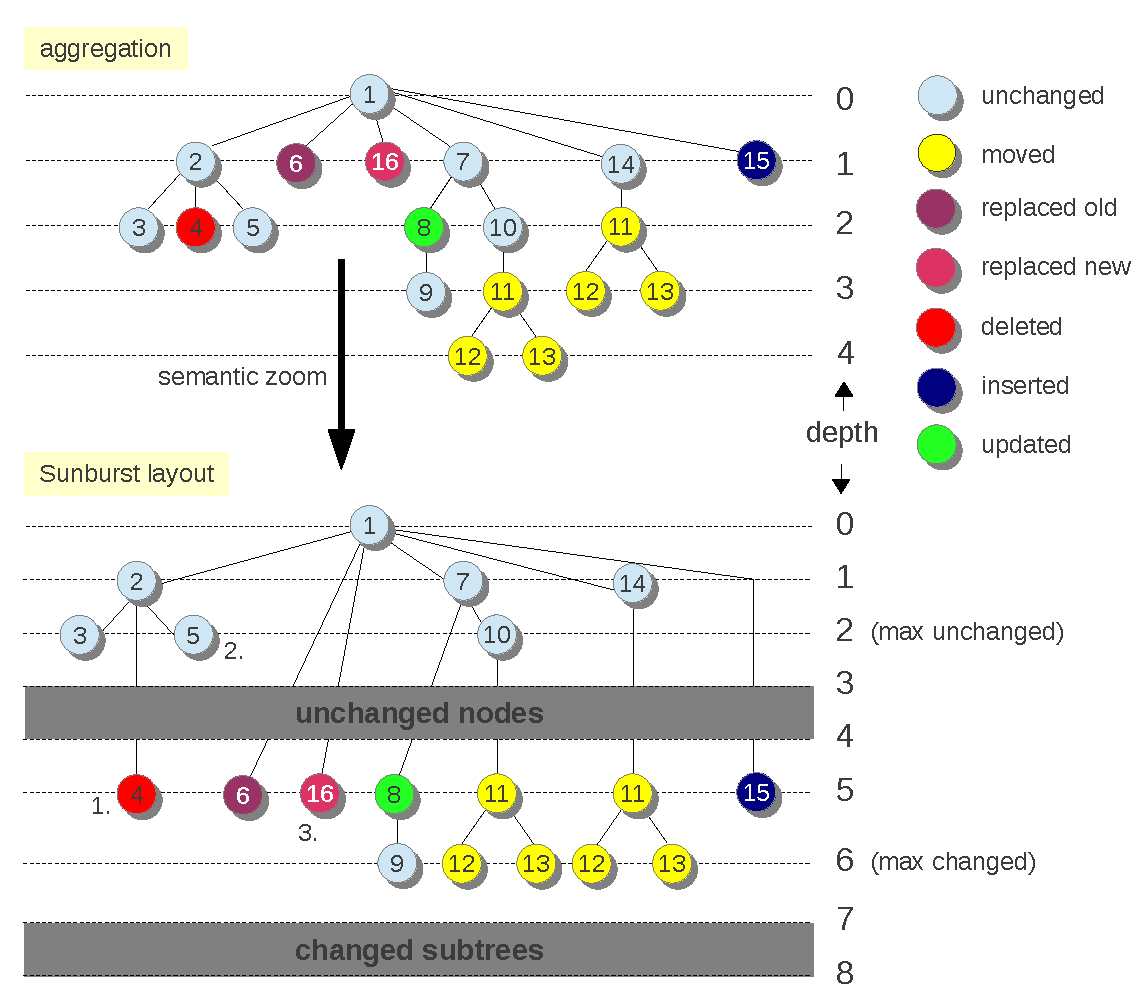
\includegraphics[width=\textwidth]
{figures/sunburst-layout}}
\caption{\label{fig:sunburst-layout} Sunburst-layout depicting changes in the depth. All nodes above the grey rectangle labeled "unchanged nodes" are unchanged whereas the area between the rectangle named "changed subtrees" includes all changed subtrees. However it also includes changed nodes below an updated node as for instance node 9.}
\end{figure}

Algorithm \ref{algo:calcDepth} determines if and how the depth must be adjusted. The first and second case is handled by the first \texttt{if}-clause, whereas the transition back to the original depth is handled by the \texttt{elseif}-clause. An instance variable \emph{mTempKey} is used to determine when to switch back. It is the node-ID of the first node in the XPath \texttt{following::}-axis which is not changed. However the variable always refers to the first node in the \texttt{following::}-axis which is changed in the second case. An \texttt{UPDATED} node most probably incorporates unchanged nodes if it is an internal \texttt{ElementNode}. In these cases we do not use the original depth of the node, but the current depth based on the tree traversal in the \texttt{Diff}-Axis which reflects the original depth plus the additional depth-difference to transform the depth of the first updated node.

\begin{algorithm}[Hhtbp]
%\SetAlgoLined
\SetKwInOut{Input}{input}\SetKwInOut{Output}{output}
\Input{int pDepth, DiffType pDiff, DiffTuple pDiffCont, int pMaxDepth, PruningType pPrune, instance variables denoted by a trailing "m" (long mTempKey, long mInitDepth)}
\Output{new depth}
\BlankLine
int depth $\leftarrow$ pDepth\;
\If{pDiff != DiffType.SAME AND pDiff != DiffType.SAMEHASH AND pDepth $\leq$ pMaxDepth + 2}{
  depth $\leftarrow$ pMaxDepth + 2\;

  int index $\leftarrow$ mIndex + mPrunedNodes + mDescendantCount\;
  boolean isOldTransaction $\leftarrow$ (pDiff == DiffType.DELETED OR pDiff == DiffType.MOVEDFROM OR pDiff == DiffType.REPLACEDOLD)\;
  DiffDepth depthCont $\leftarrow$ mDiffCont.getDepth()\;
  int depth $\leftarrow$ 0\; 
  \If{isOldTransaction == true}{
    depth $\leftarrow$ depthCont.getOldDepth()\;
  }\Else{
    depth $\leftarrow$ depthCont.getNewDepth()\;
  }

  \If{index $<$ mDiffs.size()}{
    Diff nextDiffCont $\leftarrow$ mDiffs.get(index)\;
    DiffType nextDiff $\leftarrow$ nextDiffCont.getDiff()\;
    boolean nextIsOldTransaction $\leftarrow$ (nextDiff == DiffType.DELETED OR nextDiff == DiffType.MOVEDFROM OR nextDiff == DiffType.REPLACEDOLD)\;
    DiffDepth nextDepthCont $\leftarrow$ nextDiffCont.getDepth()\;
    int nextDepth $\leftarrow$ 0\;
    \If{nextIsOldTransaction == true}{
      nextDepth $\leftarrow$ nextDepthCont.getOldDepth()\;
    }\Else{
      nextDepth $\leftarrow$ nextDepthCont.getNewDepth()\;
    }

    mTempKey $\leftarrow$ 0\;
    \If{nextIsOldTransaction == true}{
      mTempKey $\leftarrow$ nextDiffCont.getOldNodeKey()\;
    }\Else{
      mTempKey $\leftarrow$ nextDiffCont.getNewNodeKey()\;
    }
  }
}\ElseIf{(pDiff == DiffType.SAME OR pDiff == DiffType.SAMEHASH) AND pDiffCont.getNewNodeKey() == mTempKey}{
  depth $\leftarrow$ pDiffCont.getDepth().getNewDepth() - mInitDepth\;
}
return depth\;
\caption{Calculate depth}\label{algo:calcDepth}
\end{algorithm}

Besides adjusting the depth the semantic zoom requires some form of highlighting. In our case we opted for a global "distortion" which enlarges modified subtrees and shrinks subtrees of unchanged nodes. Thus, the extend of a Sunburst item depends on two variables, the \texttt{descendant-or-self}-count and the number of \texttt{modification}s in a nodes' subtree.

\begin{equation}
ext = \left\{ \begin{array}{cl}
2 \cdot \pi & \textrm{if }node\ is\ root\ node\\
parExt \cdot ((1-\alpha) \cdot descs / (parDescs - 1) \\+ \alpha \cdot mods / (parMods - 1)) & \textrm{otherwise}\end{array}\right.
\end{equation}

The modification-count in the forumla is derived from the \\ \texttt{descendant-or-self}-count added to the \texttt{modification}-count of the current node plus a constant. The addition of the \texttt{descendant-or-self}-count is needed to handle nodes, which do not contain any modifications in its subtree and the node itself is not changed, too. In order to further emphasize and enlarge subtrees with a small number of modifications a constant is added which has proven useful in empirical studies (Chapter \ref{sec::applications}). Futhermore note that if the parent node has been modified the constant must be subtracted from the parent \texttt{modification}-count in advance. Otherwise the equation will not work.

The two variables are computed in parallel to the \texttt{Diff-Axis}-traversal \\whereas the results are appended to a \texttt{BlockingQueue}, which is a thread safe queue designed for producer/consumer relationships. Modifications for the root node are gathered while observing diff-tuples, thus the modifcation-count does not need to be computed afterwards as for the other nodes in the agglomerated tree-structure. A simple heuristic determines depending on a depth-threshold if tasks are executed in the calling thread instead of another thread, as context switches for very small subtrees are too costly. Observe that the added descendant-count for each node can not be used, because the aggregated tree-structure is traversed which incorporates deleted and moved nodes. Algorithm \ref{algo:descModCount} depicts how the two variables are derived from traversing the diff-datastructure at a specified index until the depth of a diff in the agglomerated tree-structure either is less than or equal to the start depth or no more diff-tuples are following. Note that the depth depends on the diff-type. In case of a \texttt{DELETED}, \texttt{MOVEDFROM} or \texttt{REPLACEDOLD} diff-type the depth of the node in the older revision is used, otherwise the depth of the node in the new revision. Furthermore recapitulate that the depths are computed by the ID-based diff-algorithm instead of stored directly in the node by Treetank.

\begin{algorithm}[Hhtbp]
%\SetAlgoLined
\SetKwInOut{Input}{input}\SetKwInOut{Output}{output}
\Input{int pIndex, List pDiffs}
\Output{CONSTANT\_FACTOR * diffCounts, descendantCounts, subtract}
\BlankLine
int index $\leftarrow$ pIndex\;
DiffTuple diffCont $\leftarrow$ pDiffs.get(index)\;
DiffType diff $\leftarrow$ diffCont.getDiff()\;
int rootDepth $\leftarrow$ diffCont.getDepth().getNewDepth()\;
\If{diff == DiffKind.DELETED OR diff == DiffKind.MOVEDFROM OR currDiff == DiffType.REPLACEDOLD}{
  rootDepth $\leftarrow$ diffCont.getDepth().getOldDepth()\;
}

int diffCounts $\leftarrow$ incrDiffCounter(index)\;
int descendantCounts $\leftarrow$ 1\;
boolean subtract $\leftarrow$ false\;
diffCounts = incrDiffCounter(index)\;
index $\leftarrow$ index + 1\;

\If{diffCounts == 1 AND index $<$ mDiffs.size()}{
  DiffTuple cont $\leftarrow$ mDiffs.get(index)\;
  int depth $\leftarrow$ cont.getDepth().getNewDepth()\;
  \If{cont.getDiff() == DiffType.DELETED OR cont.getDiff() == DiffType.MOVEDFROM OR currDiff == DiffType.REPLACEDOLD}{
    depth $\leftarrow$ cont.getDepth().getOldDepth()\;
  }
  \If{depth == rootDepth + 1}{
    \tcp{Current node is modified and has at least one child.}
    subtract $\leftarrow$ true\;
  }
}

boolean done $\leftarrow$ false\;
\While{!done AND index $<$ mDiffs.size()}{
  DiffTuple currDiffCont $\leftarrow$ mDiffs.get(index)\;
  DiffType currDiff $\leftarrow$ currDiffCont.getDiff()\;
  DiffDepth currDepth $\leftarrow$ currDiffCont.getDepth()\;
  int depth $\leftarrow$ currDepth.getNewDepth()\;
  \If{currDiff == DiffType.DELETED OR currDiff == DiffType.MOVEDFROM OR currDiff == DiffType.REPLACEDOLD}{
    depth $\leftarrow$ currDepth.getOldDepth()\;
  }
  \If{depth $\leq$ rootDepth}{
    done $\leftarrow$ true\;
  }
  \If{!done}{
    descendantCounts $\leftarrow$ descendantCounts + 1\;
    \If{currDiff != DiffKind.SAME AND currDiff != DiffKind.SAMEHASH}{
      diffCounts $\leftarrow$ diffCounts + 1\;
    }
    index $\leftarrow$ index + 1\;
  }
}
\caption{Derives \texttt{descendant-or-self}-count as well as the \texttt{modification}-count}\label{algo:descModCount}
\end{algorithm}

\subsubsection{Filtering/Pruning}
Providing an initial Sunburst overview of huge tree-struc\-tures in reasonable time, ranging from a few seconds to a few minutes, requires pruning techniques to filter nodes of no or least interest. Therefore three types of filtering are provided. Changes in a nodes' subtree are always guaranteed to be visible. The following screenshots in this section are related to Fig. \ref{fig:without-pruning} which depicts the same tree comparison in the SunburstView without filtering nodes.

\begin{figure}[tb]
\center{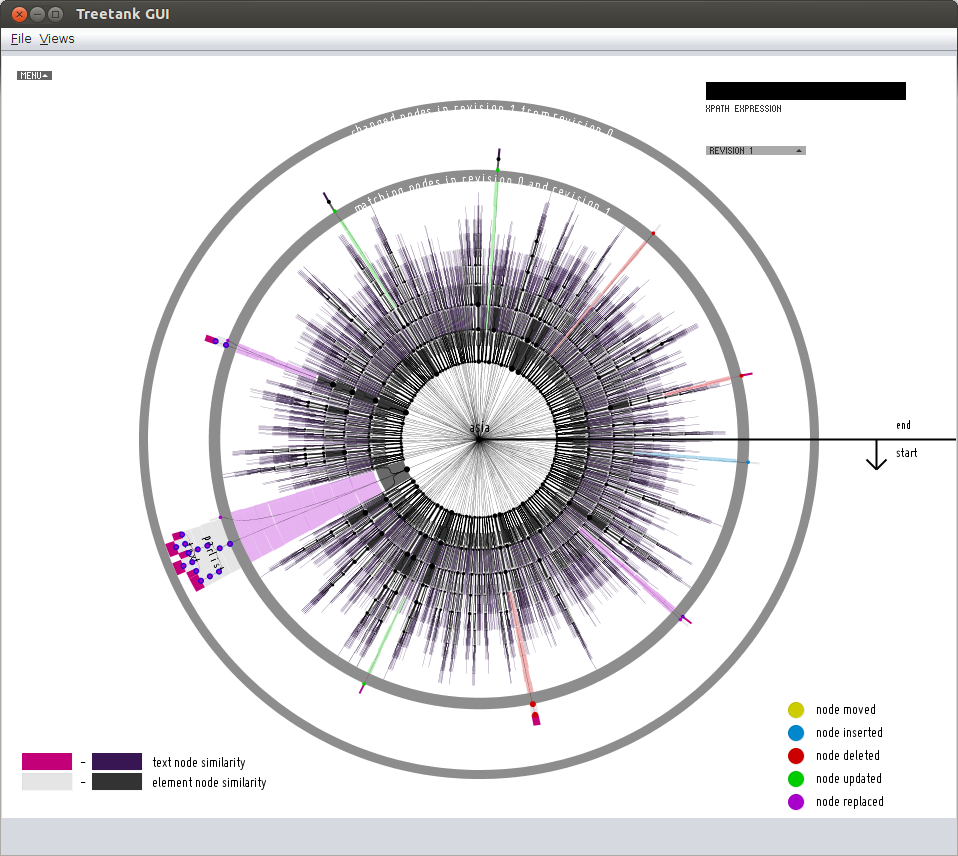
\includegraphics[width=\textwidth]
{figures/without-pruning}}
\caption{\label{fig:without-pruning} Comparison without pruning.}
\end{figure}

\begin{itemize}
\item \emph{by itemsize} Sunburst items which have no changes in its subtree and are too thin to perceive individually or too thin to select even with the fisheye transformantion are pruned based on a predefined threshold-value. An example is depicted in Fig. \ref{fig:pruned-by-itemsize}. This type of filtering is useful wherever nodes which do not differ are of value but depicting the whole tree will not add any significant value and/or does not . It considerably speeds up the generation of the Sunburst items in large tree-structures, however it does not effect the diff-calculation. Furthermore if a new node is selected to drill down into the tree the item creation must be redone, based on the \texttt{Diff}-axis, thus no optimization which just creates new items based on the initial set with adjusted angles can be used. The \texttt{descendant-or-self}-count as well as the \texttt{modification}-count must be recalculated. 

\begin{figure}[tb]
\center{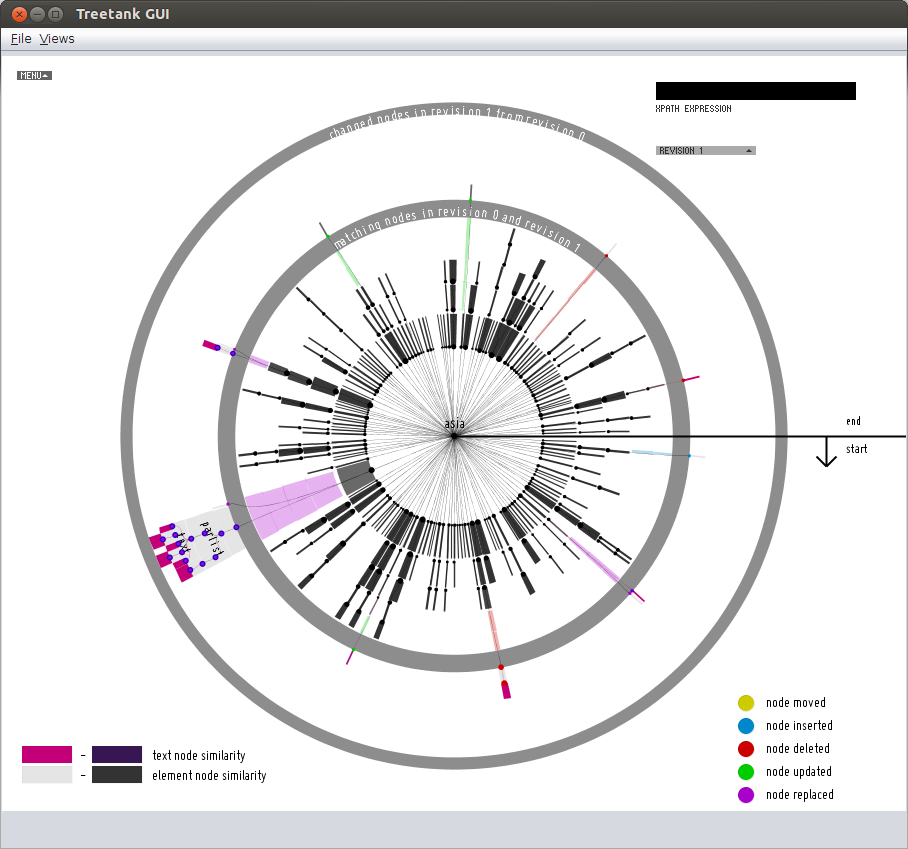
\includegraphics[width=\textwidth]
{figures/itemsize-pruned}}
\caption{\label{fig:pruned-by-itemsize} Pruned by itemsize.}
\end{figure}

\item \emph{by hash-based diff-algorithm} The diff-algorithm is called with the option to utilize persisted hashes which are created for every resource based on a database-configuration paramete. Per default rolling hashes which are very fast are used. The hashes of ancestor-nodes are recomputed for all edit-operations. As described in Chapter \ref{sec::differences} everytime the hash values during node-comparisons are identical the whole subtree is skipped in both revisions. Thus, only items are created for nodes, which contain changes in their subtree including subtree-roots for which identical hash-values are determined (Fig. \ref{fig:pruned-by-hash}). This type of pruning is especially useful for large tree-structures, whereas in contrast to the pruning by itemsize it speeds up the diff-computation as well as the item creation, as in both cases subtrees of nodes with the same hashes are skipped. However, it might be that more items in comparison with the itemsize-based approach are created as nodes with identical hash-values are always included.

\begin{figure}[tb]
\center{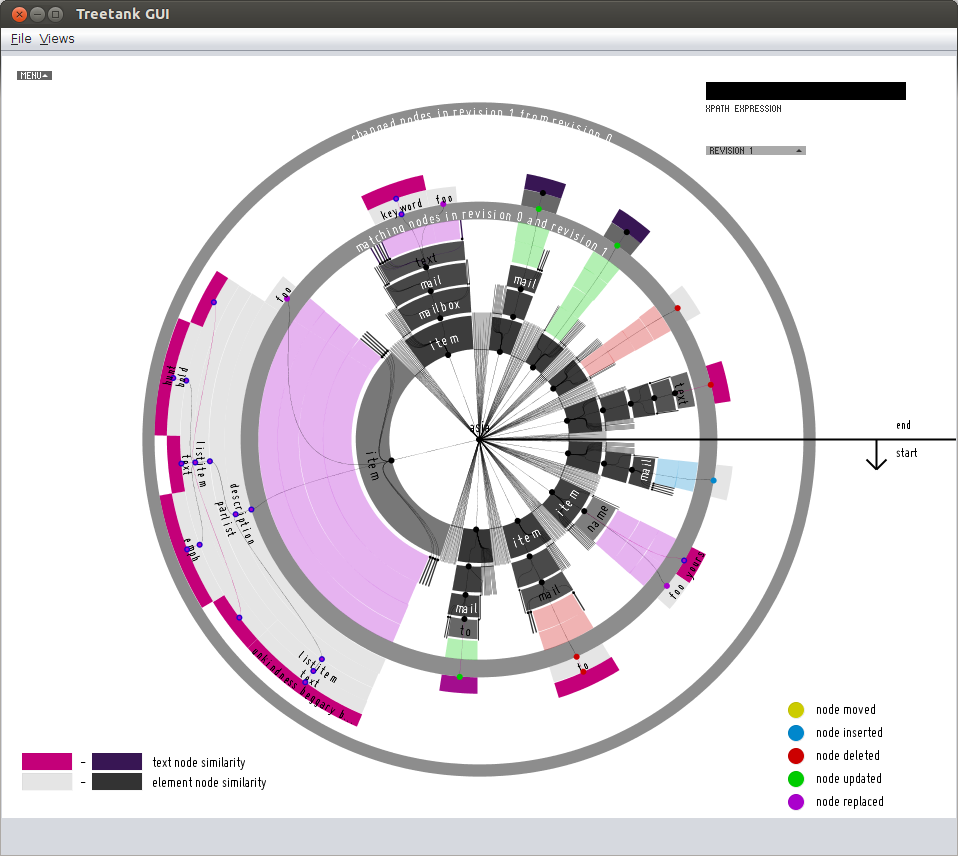
\includegraphics[width=\textwidth]
{figures/diff-pruned}}
\caption{\label{fig:pruned-by-hash} Pruned by same hashes.}
\end{figure}

\item \emph{by hash-based diff-algorithm without nodes which have the same hash} This type of pruning is closely related to the filtering-method described above. In addition to filtering nodes in the subtree of nodes which have the same hash-value, items for this type of "difference" are not created at all. A consequent is a much better readability of the differences in case of many consecutive nodes with the same hash-value (Fig. \ref{fig:pruned-by-hash-without-samehashes}).

\begin{figure}[tb]
\center{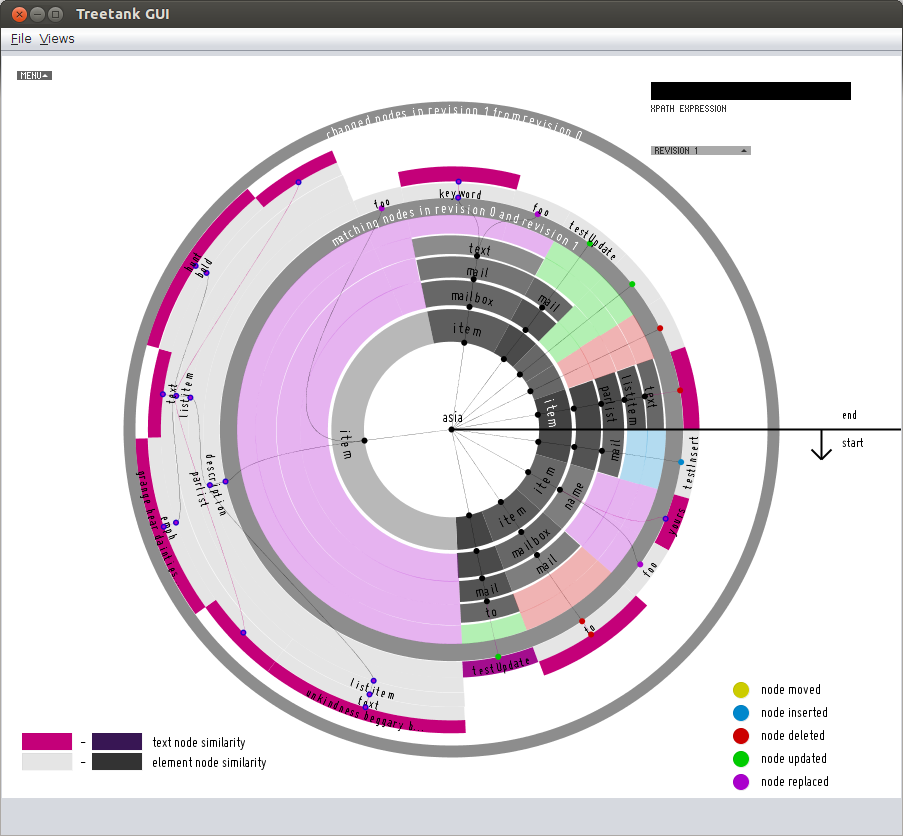
\includegraphics[width=\textwidth]
{figures/diff-without-samehashes-pruned}}
\caption{\label{fig:pruned-by-hash-without-samehashes} Pruned by hash-value without building items for nodes with same hash-values.}
\end{figure}
\end{itemize}

Usually the maximum depth of unchanged nodes in the aggregated tree-structure is computed in parallel using a \texttt{BlockingQueue} if more than two cores are available taking diff-tuples off the head of the queue during observation. However, all filtering types require postprocessing as maximum depth nodes might either be within the subtree of an unchanged node and in case of the itemsize-based filtering might be too thin regarding a threshold value. Thus, the maximum depth must be recomputed and the depth of unchanged nodes must be adapted and reduced accordingly. Note, that otherwise too much space would be wasted as the root of changed nodes is plotted at \emph{maxDepth of unchanged nodes} plus two.

Having described several filtering methods and briefly meantioned a general zooming/panning technique based on affine transformations which is inherited from the \emph{SunburstView} layout depicting one revision. Besides it is of the utmost importance to enlarge specific subtrees in the layout itself. The next section gives some insight on how to the selection of new root-nodes to dig deeper into the tree-structure is handled.

\subsubsection{Zooming / Details on demand} 
Supporting analyists with the ability to dig deeper into the tree-structure for most but the tiniest tree-structures is crucial. Thus we support the selection of a new root node by a mouse-click on the desired item. In our first version this triggered the recalculation of the diffs for the nodes' subtree as well as the the maximum depth of unchanged nodes, the modification- and the descendant-count for each node in the subtree to build new enlarged items. The former items are pushed on a stack to support a simple undo-operation.

However due to unnecessary recalculations despite in case of the item-based pruning our simplyfied approach just recalculates the maximum depth of the unchanged nodes in parallel utilizing all available cores and subsequently builds new items based on a simple upscaling.

Having described the new Sunburst-layout tailored to comparison of tree-structures with all available pruning methods and the ability to select a new root-node in detail the next section describes how the similarity score between different types of nodes is measured, which is used to map colors to the items.

\subsubsection{Similarity measures}
Similarities for \texttt{Element}- and \texttt{Text}-nodes are measured differently. The only inner nodes of an XML-document are element nodes (which can also be leaf nodes).

\texttt{Element}-node similarity is measured based on overlapping subtrees. Consider the comparison of tree-structures T1 and T2. The similarity score for an element in the aggregated tree-structure $T_{aggr}$ is defined as

\begin{equation}
Sim(node_{T_{aggr}}) = \frac{descs(node_{T_{aggr}}) - mods(node_{T_{aggr}})}{descs(node_{T_{aggr}})}
\end{equation}

The similarity score is normalized between $[0, 1]$. The nodes of type\\ \texttt{INSERTED/DELETED/REPLACED} always are scored 0 as they do not have any equivalent in the other tree. In case of \texttt{SAME}-nodes the similarity depends on overlapping subtree-structures. If no modifications are in the subtree the score is 1. \texttt{UPDATED} nodes are counted as a modifications and therefore add to the dissimilarity.

\texttt{Text}-nodes are leaf nodes which therefore have no child. The similarity score is defined as

\begin{equation}
Sim(node_{T_{aggr}}) = \left\{ \begin{array}{cl}
Levenshtein(node_{T_{1}}, node_{T_{2}}) & \textrm{if }node\ is\ \texttt{UPDATED}\\
0 & \textrm{if }node_{T_{aggr}}\ is \texttt{INSERTED}\\
  & \texttt{/DELETED/REPLACED}\\
1 & \textrm{otherwise}\end{array}\right.
\end{equation}

Note that the similarity score is computed based on the diff-tuple which incorporates both nodeKeys. In case of an \texttt{UPDATED} \texttt{text}-node the Levenshtein algorithm is used, which defines a similarity score based on per-character edit-operations to change one string-value into the other one and is normalized between 0 (no similarity) and 1 (same string-value). 

\subsection{Querying}
XPath 2.0 queries are currently partly supported by our XPath 2.0 engine. We also examined our Saxon binding, which was surprisingly rather slow. However we did not measure time differences which is out of scope of this thesis. Future work might include a Brackit\cite{Brackit} binding which is a "flexible XQuery-based query engine" developed at the TU Kaiserslautern. In contrast to Saxon it is specifically designed to work on top of databases and adding specific indexes for instance will be easy. However this feature is currently reevaluated.

We provide query capabilities on top of the agglomerated tree-structure and therefore query both compared revisions in parallel. The items are sorted by node-ID in parallel. Once all query results have been collected they are also sorted (the result is a sequence of node-IDs). A subsequent traversal of the items highlights items which are included in the query results.

\subsection{Visualization of moves}
Hierarchical Edge Bundles\cite{Bundles} are used to avoid visual clutter of subtree moves. The technique creates a path up to but usually not including the Lowest Common Ancestor (LCA) of a source-node down to the destination-node. The path is used to define control points for plotting a curve.

The LCA is defined as:

\begin{equation}
lca(a{,} b) = min\{c|a \prec c, b \prec c\}
\end{equation}

A simple algorithm computes the LCA through the \texttt{push()}-operation on two stacks following the first node (moved from) and the second node (moved to) up to the root-node. In a next step the two stacks are processed in a loop using \texttt{pop()} as long as identical node-IDs are found. The LCA is the first node-pair for which the node-IDs do not match.

Fig. \ref{fig:moves} illustrates two move-operations on a subtree in a shakespear XML-document.

\begin{figure}[tb]
\center{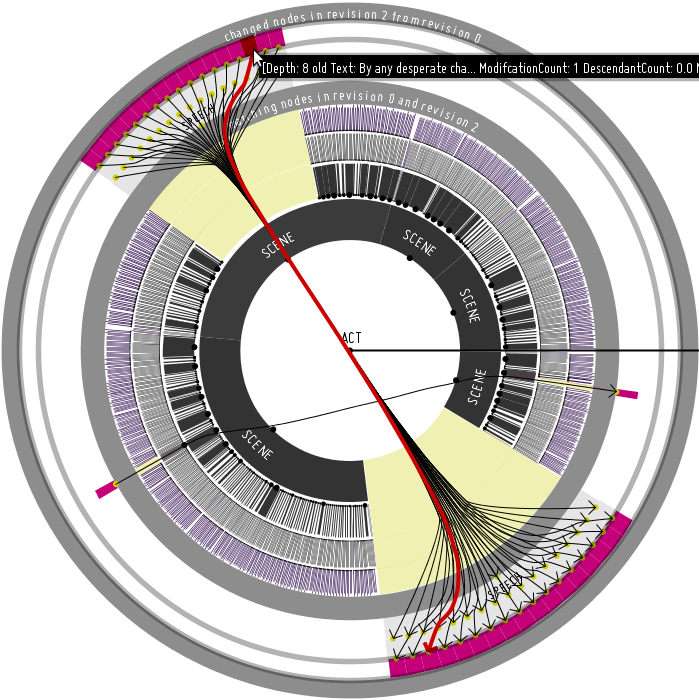
\includegraphics[width=\textwidth]
{figures/moves-cut}}
\caption{\label{fig:moves} Moves visualized using hierarchical edge bundles.}
\end{figure}

Despite comparing two tree-structures we furthermore aim to support a broad overview about the changes (and similarities) of currently at most five trees.

\subsection{Small multiple}\label{subsec::smallmultiple}
Small multiple visualizations of the \emph{SunburstView} are therefore used to provide an overview about the changes between several tree-structures, whereas the restriction of comparing five tree-structures is merely an implementation detail which in future versions will be configurable. Two variants based on same-titled well known revisioning strategies are described next.

\begin{itemize}
\item \emph{differential} The differential variant displays changes related to a base revision. This is especially useful if several tree-structures have to be compared to a common base revision. The direction is clockwise. That is the upper left corner displays a SunburstView comparison between revision 0 and 1 (if zero is the base revision which is loaded), the right upper corner displays changes between revision 0 and revision 2 et cetera (Fig. \ref{fig:smallmultiple-differential}).

\begin{figure}[tb]
\center{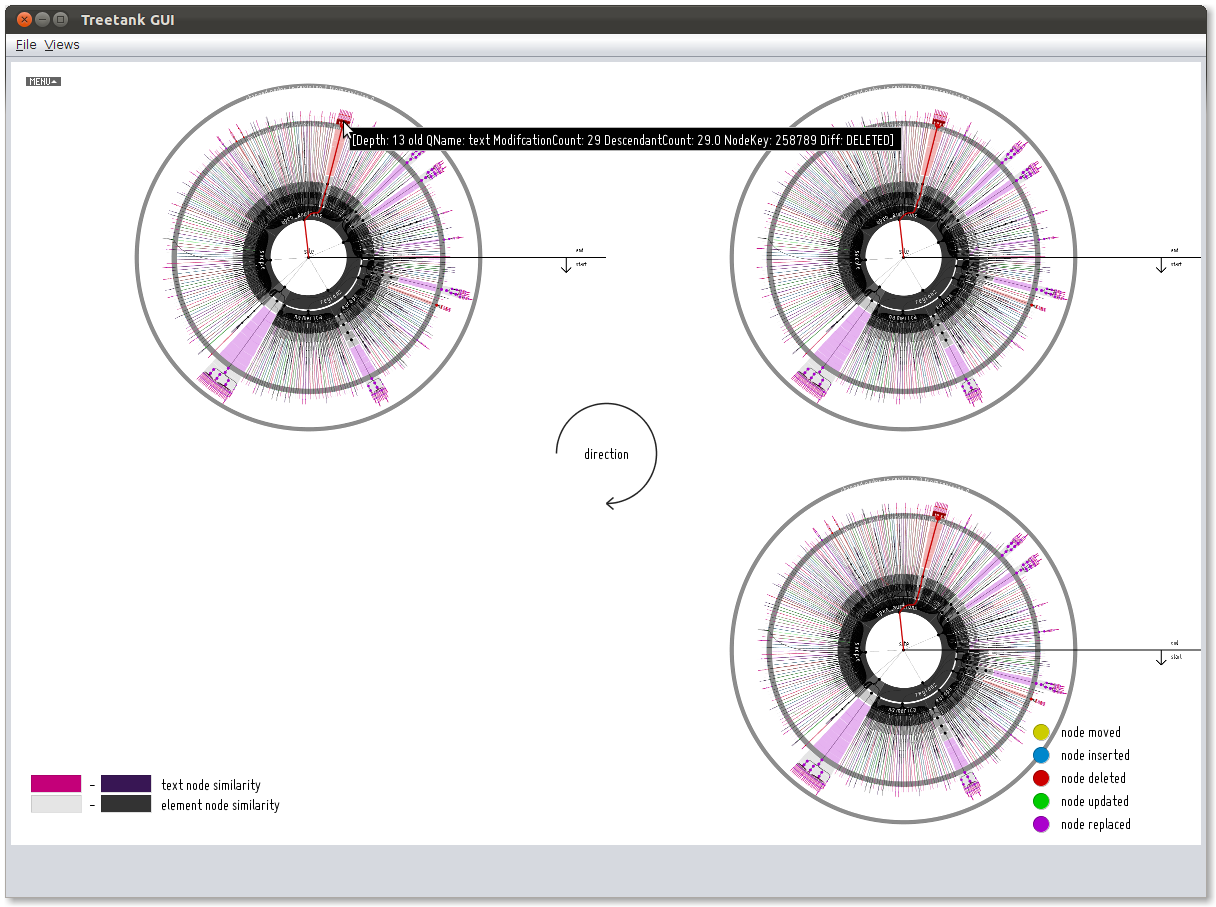
\includegraphics[width=\textwidth]
{figures/smallmultiple-differential}}
\caption{\label{fig:smallmultiple-differential} Small multiple - differential variant.}
\end{figure}

\item \emph{incremental} The incremental variant displays changes related to the last compared revision in increasing order. Suppose we have loaded revision 2, then in the upper left corner revision 2 and 3 is compared, the upper right corner contains the comparison between revision 3 and 4 et cetera (Fig. \ref{fig:smallmultiple-incremental}).

\begin{figure}[tb]
\center{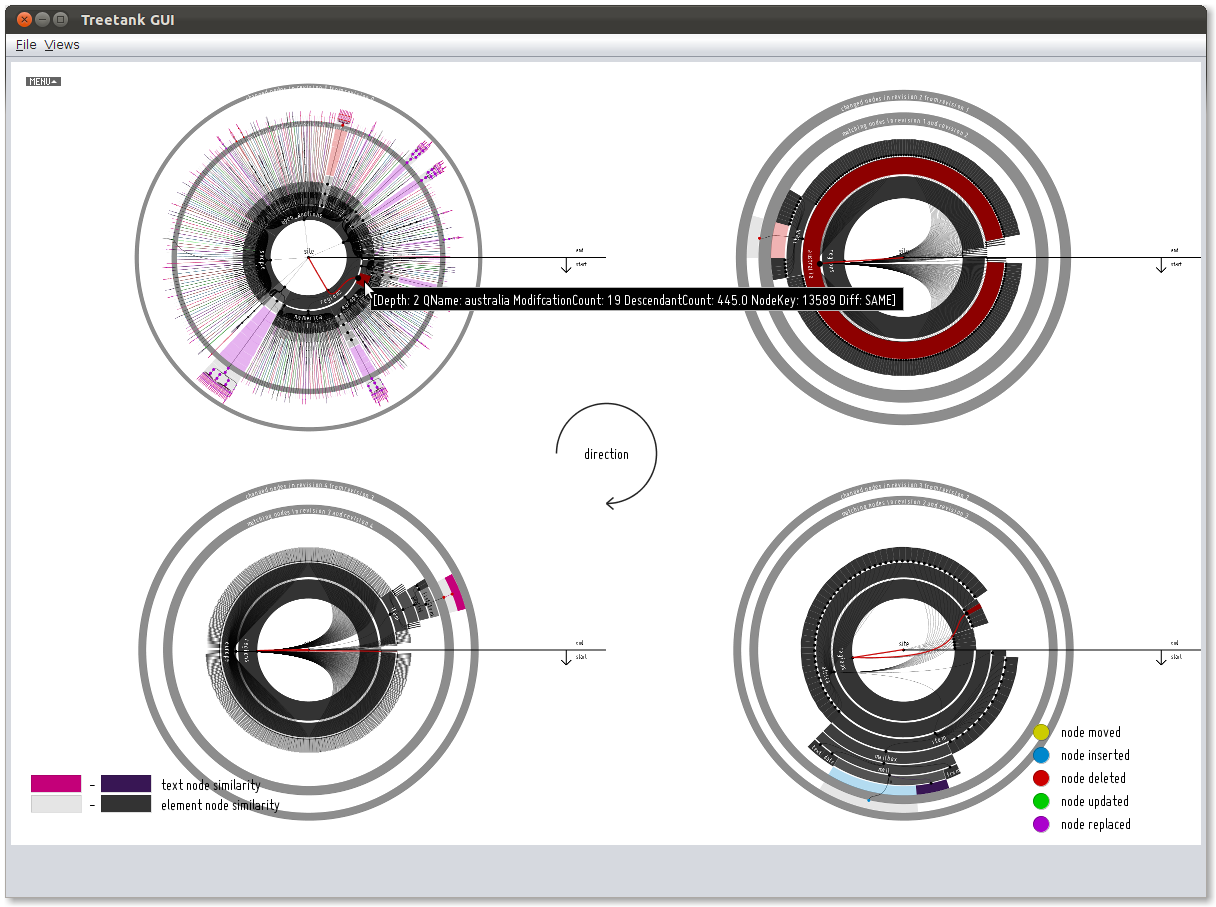
\includegraphics[width=\textwidth]
{figures/smallmultiple-incremental}}
\caption{\label{fig:smallmultiple-incremental} Small multiple - incremental variant.}
\end{figure}
\end{itemize}

The implementation parallizes the computation of the small multiple and stores each Sunburst-visualization in an offscreen image, which is appended to a list in the view. This list must be sorted after all visualizations have been computed accoring to a revision which is saved along with the buffered offscreen image to support the clockwise order. The items of each visualization are saved in a simple datastructure in the model to support highlighting of items on mouse over through brushing and linking. The technique is illustrated in Fig. \ref{fig:smallmultiple-differential} and \ref{fig:smallmultiple-incremental}. Items are highlighted in red just like in the SunburstView but the same item based on a node-ID equivalence relation is linked and highlighted in all small visualizations.

The three variants support all filtering methods described earlier. However in the case of the hybrid view only the itemsize-based pruning is of any value. Otherwise most items would not be plotted in subsequent revisions.

Next we provide a short asymptotic runtime- and space-analysis backed by performance measures.

\subsection{Runtime/Space analysis and scalability of the ID-based diff}
The runtime of the algorithm currently is bound by determining the number of descendants and modifications in the agglomerated tree-structure for each node. The runtime complexity thus is $O(n^2)$ whereas $n$ is the sum of changed and unchanged nodes between two trees $T1$ and $T2$. However by storing the diff-tuples which only include the depth of the two compared nodes to form a very simple tree-structure we are limited to a preorder traversal. Building a more sophisticated tree-structure based on pointers or sequences denoting child nodes for instance in an in-memory Treetank structure will support a subsequent postorder traversal to determine the number of descendants and modifications for each node reducing the runtime to $O(n)$. Due to using Java7 which is not available for OS X we were not able to measure the performance on computers with four or more cores. However, counting the subtree-size and modifications is started in parallel to building Sunburst items which consumes these through a Java \texttt{BlockingQueue}. The \texttt{descendant-count/subtree-size} of the root-item (plus one) is the size of the accumulated List or Map of diff-tuples observed from the ID-based diffing algorithm and thus does not need to be computed. The \texttt{modification-count} of the root-item is also determined on the fly while observing diff-tuples. Thus we assume adding more cores will speed up the creation of the items considerably as tree-structures often times are rather flat and have a large fan-out instead of being deep with high average levels/depths of the nodes, especially considering document-centric XML \cite{ronnau2009efficient}. Fig. \ref{fig:gui-performance} shows performance measures, the average of ten runs of the Sunburst-visualization on an 11MiB-document and an 111MiB-document of the XMark-benchmark.  The documents are identical to the documents used in Chapter \ref{sec::differences} for benchmarking. Thus we randomly modified the instances after every 1000st node in the 11Mib-document and after every 10000st node in the 111MiB-document. The hardware used is also identical (Core 2 Duo 2666Mhz, 4Gb RAM). It is obvious that the exponential growth in case no pruning is enabled is unacceptable. Showing the 111MiB-document without pruning lasted too long (> 15min for each run) such that we aborted the execution. By reducing the number of Sunburst-items which have to be created considerably each one of the pruning-mechanisms reduces the runtime tremendously. Usually the number of Sunburst-items to create is reduced so much that the exponential time to compute the modifications in each nodes' subtree plus the subtree-size itself is not measurable and the runtime reduces to a linear scale. Furthermore as we were not able to measure the impact of parallelizing this task with four and more cores it might also considerably speed up the computation in the general case without pruning. We assume that the context switches with only one or two cores in fact slow down the computation. 

Fig \ref{fig:gui-performance-movedet} shows benchmarking results comparing the runtime of the fastest pruning, pruning-by-hashes without creating items for identical hashes with move-detection enabled and disabled. We are able to determine that the move-detection usually is fast. Asymptotically it is bound by the size of the agglomerated tree-structure $n$, $O(n)$.

In summary we are able to conclude that the hash-based-pruning without creating Sunburst items is by far the fastest and that the move-detection usually does not inhibit the runtime of our algorithms considerably. Furthermore it is required to use pruning whenever the exponential time required to compute subtree-sizes and modifications therein significantly inreases due to a large aggregated tree. Adding more CPUs however should decrease the runtime as the computation of subtreesizes and modifications therein are computed in parallel.

\begin{figure}[tb]
\center{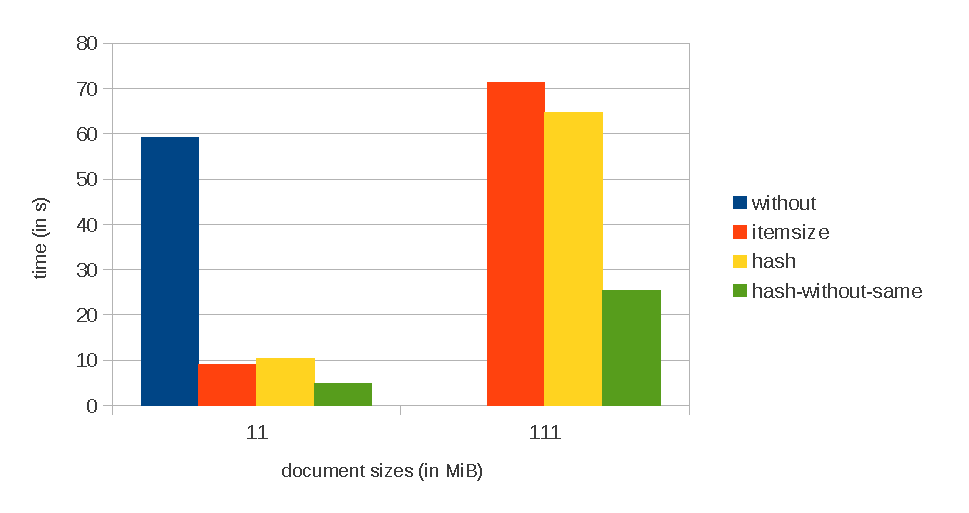
\includegraphics[width=\textwidth]
{figures/gui-performance}}
\caption{\label{fig:gui-performance} GUI-performance.}
\end{figure}

\begin{figure}[tb]
\center{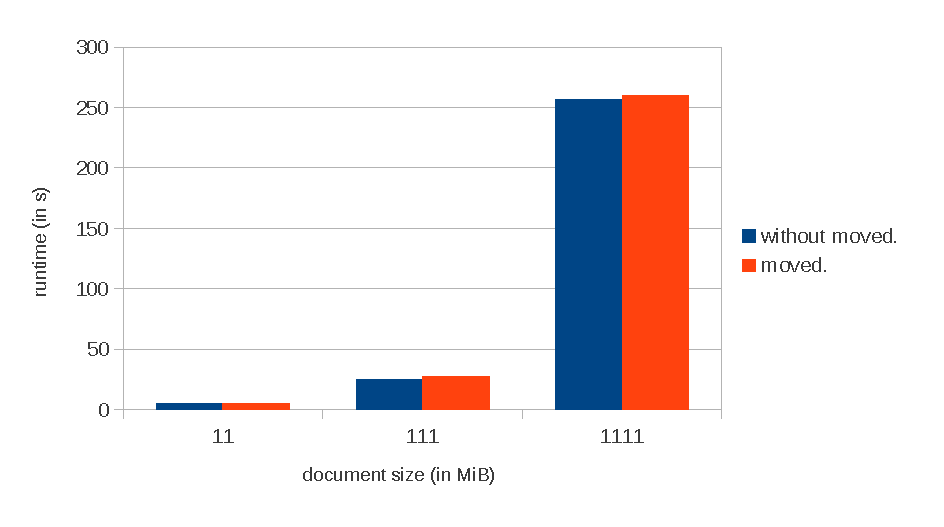
\includegraphics[width=\textwidth]
{figures/gui-performance-movedet}}
\caption{\label{fig:gui-performance-movedet} GUI-performance using hash-based pruning without adding identical hash-values and move-detection enabled/disabled.}
\end{figure}

\begin{table}[tb]
\centering 
\begin{tabular}[r]{|l|c|c|c|} 
\hline
& \textbf{1000mods} & \textbf{5000mods} & \textbf{10000mods}\\
\hline
\hline
\textbf{min} & 36265.14 & 35717.34 & 33948.96\\
\hline
\textbf{max} & 52459.38 & 61860.29 & 44451.06\\
\hline
\textbf{average} & 39167.75 & 37650.67 & 36579.37\\
\hline
\end{tabular}
\label{chap3:comparsion}
\vspace{0.5em} 
\caption{Comparsion of different modification-schemas of a 111 MiB XMark instance (change every 1000st, 5000st and 10000st node).}
\end{table}

\subsection{Conclusion and Summary}
We have introduced a multitude of visualizations ranging from a simple \emph{TextView} displaying syntax highlighted serialized XML in the viewport and appends new text during scrolling to a \emph{SunburstView} and several \emph{Smallmultiple} variants based on the \emph{SunburstView}. Our main contribution is a new Sunburst layout based on the idea of a semantic zoom, which places all changed nodes prominently between two rings and distorts the whole layout to enlarge subtrees which include changed nodes and to shrink whole subtrees with no changes. 

Moreover three filtering techniques have been described which especially facilitate the analysis of large tree-structures. Pruning by itemsize is useful if changed \emph{and} and unchanged nodes are of importance speeding up the creation of items considerably. However it does not affect the diff-computation. Thus, we introduced hash-based filtering techniques, which utilize the diff-algorithm with the optimization to skip the traversal of subtrees of nodes with same hash-values. These filtering types reduce the number of items even more. Additionaly the diff-computation is faster due to the optimization. Note that changed nodes are never skipped and therefore only nodes of no or less interest are lost and not displayed.

Move-detection is enabled on demand. Furthermore inserted/deleted subtrees in a row are summarized as replace-operations.

In addition to the \emph{TextView} and \emph{SunburstView} small multiple variants support the comparison of multiple trees ($> 2$). The number of comparsions is only limited by our implementation (which is only an implementation-detail) and the available screen space. Note, that the small multiples currently use too much unused screen space due to storing the whole visualization except the legends and menus in an offscreen image. As the with of the main GUI-window usually is not squarified the space used for menu-components and legends in the \emph{SunburstView} is multiplied and wasted. However this is merely an implementation detail which will be fixed in a future version. The filtering techniques are also available. In case of severe variations of the number of differences the incremental variant benefits the most.








